% Báo cáo giữa kỳ - Phân tích và Khai phá dữ liệu. Biên dịch: tectonic main.tex (XeTeX)
\documentclass[11pt,a4paper]{article}
\usepackage{fontspec}
\setmainfont{texgyretermes}[Extension=.otf,UprightFont=*-regular,BoldFont=*-bold,ItalicFont=*-italic,BoldItalicFont=*-bolditalic]
\setsansfont{texgyreheros}[Extension=.otf,UprightFont=*-regular,BoldFont=*-bold,ItalicFont=*-italic,BoldItalicFont=*-bolditalic]
\setmonofont{texgyrecursor}[Extension=.otf,UprightFont=*-regular,BoldFont=*-bold,ItalicFont=*-italic,BoldItalicFont=*-bolditalic,Scale=0.88]
\usepackage[a4paper,left=2.4cm,right=2.4cm,top=2.4cm,bottom=2.4cm]{geometry}
\usepackage{graphicx,booktabs,tabularx,longtable,array,amsmath,amssymb,xcolor,enumitem,placeins,fancyhdr,setspace}
\usepackage[font=small,labelfont=bf,labelsep=period]{caption}
\usepackage{tikz}
\usetikzlibrary{arrows.meta,positioning,calc}
\usepackage[colorlinks=true,linkcolor=blue!50!black,urlcolor=blue!50!black,citecolor=blue!50!black]{hyperref}

\renewcommand{\figurename}{Hình}
\renewcommand{\tablename}{Bảng}
\renewcommand{\contentsname}{Mục lục}
\renewcommand{\refname}{Tài liệu tham khảo}
\renewcommand{\abstractname}{Tóm tắt}
\renewcommand{\arraystretch}{1.15}
\setlist{nosep,leftmargin=1.4em}
\setstretch{1.08}
\setlength{\parskip}{3pt}
\emergencystretch=3em
\graphicspath{{../../figures/02_understanding/}{../../figures/03_preprocessing/}{../../figures/03_preprocessing_eval/}{../../figures/04_preparation/}{../../figures/05_clustering/}}

\definecolor{cTeal}{HTML}{2E9C8A}
\definecolor{cViolet}{HTML}{9A4D8E}
\definecolor{cBlue}{HTML}{3775BA}
\definecolor{cGray}{HTML}{8C8C8C}

\makeatletter
\def\var@iter#1{\ifx#1\@nil\else\var@char#1\expandafter\var@iter\fi}
\def\var@char#1{\ifx#1_\_\allowbreak\else#1\fi}
\newcommand{\var}[1]{\texttt{\var@iter#1\@nil}}
\makeatother
\newcommand{\CI}[2]{[#1; #2]}

\pagestyle{fancy}
\fancyhf{}
\fancyhead[L]{\small Phân cụm khách hàng thương mại điện tử}
\fancyhead[R]{\small MSSV 24022433}
\fancyfoot[C]{\small\thepage}
\renewcommand{\headrulewidth}{0.3pt}

\begin{document}

\begin{titlepage}
\centering
{\small Mã nguồn: \href{https://github.com/quanai06/midterm_datamining}{github.com/quanai06/midterm\_datamining}\quad|\quad Nhật ký cộng tác AI: \href{https://github.com/quanai06/midterm_datamining/blob/main/docs/ai_log.md}{docs/ai\_log.md}}\\[1.0cm]
{\large ĐẠI HỌC QUỐC GIA HÀ NỘI\\ TRƯỜNG ĐẠI HỌC CÔNG NGHỆ}\\[1.2cm]
{\Large \textbf{BÁO CÁO GIỮA KỲ}}\\[0.3cm]
{\large Môn: Phân tích và Khai phá dữ liệu}\\[1.8cm]
{\LARGE \textbf{Phân nhóm khách hàng thương mại điện tử\\[2pt] trên dữ liệu giả lập}}\\[0.6cm]
{\large Từ thiết kế dữ liệu, hiểu và xử lý dữ liệu đến phân cụm và đánh giá}\\[2.4cm]
\begin{tabular}{rl}
Sinh viên: & \textbf{Lê Hoàng Quân}\\
Mã sinh viên: & \textbf{24022433}\\
Lớp: & \textbf{K69A-AI3}\\
\end{tabular}\\[2.6cm]
{\normalsize Hà Nội, tháng 11 năm 2026}
\end{titlepage}

\begin{abstract}
\noindent Báo cáo xây dựng một quy trình khai phá dữ liệu hoàn chỉnh cho bài toán phân nhóm khách hàng thương mại điện tử (học không giám sát):
sinh dữ liệu giả lập có cấu trúc hành vi tiềm ẩn ($N=260$, 14 thuộc tính, nhiễu, 15 khách có ngoại lai, 3 cột thiếu giá trị), hiểu dữ liệu, tiền xử lý,
chuẩn bị dữ liệu và phân cụm. Dữ liệu trước xử lý và sau xử lý được so sánh bằng K-Means trên cùng 260 khách.
Với $k=4$, ARI so với phân khúc ẩn tăng từ $0{,}611$ \CI{0,515}{0,708} lên $0{,}745$ \CI{0,658}{0,833}; khi $k$ được chọn bằng Silhouette,
dữ liệu thô cho $k=7$ (ARI $0{,}434$) còn dữ liệu đã chuẩn bị chọn đúng $k=4$ (ARI $0{,}745$) và ổn định hơn rõ rệt.
Đóng góp riêng của bước chuẩn bị tại $k=4$ chưa chứng minh được ($+0{,}044$, khoảng tin cậy chứa 0); bằng chứng nằm ở việc chọn $k$ và độ ổn định.
Phân khúc ẩn chỉ dùng để đánh giá, không dùng để chọn tham số; các kết quả không thuận lợi được nêu cùng với kết quả.
\end{abstract}

\tableofcontents
\newpage

\section{Bài toán và phạm vi}
\label{sec:intro}

\subsection{Bài toán cần giải quyết}
Một sàn thương mại điện tử có tập khách hàng với các đặc điểm (tuổi, thiết bị, hạng thành viên, ngành hàng ưa thích) và hành vi (lịch sử mua hàng, chi tiêu, mức dùng khuyến mãi, hành vi duyệt, mức tương tác với nền tảng).
Doanh nghiệp muốn chia khách thành một vài nhóm sao cho khách trong cùng nhóm có hành vi giống nhau và khác với các nhóm còn lại, để chăm sóc, giữ chân và tiếp thị phù hợp với từng nhóm (ví dụ khách giá trị cao, khách chủ yếu săn khuyến mãi,
khách mua không thường xuyên, khách chủ yếu duyệt mà không mua). Không có nhãn nhóm sẵn có, nên đây là bài toán \emph{phân cụm} (học không giám sát).

Khó khăn nằm ở chất lượng dữ liệu: nhiễu đo lường, ngoại lai (cần phân biệt lỗi nhập liệu với khách cực trị có thật), giá trị thiếu, phân phối lệch phải, thuộc tính trùng lặp và dữ liệu hỗn hợp số/thứ tự/định danh với thang đo rất khác nhau.
Các vấn đề này làm méo khoảng cách giữa các khách hàng, mà thuật toán phân cụm dựa vào chính khoảng cách đó. Câu hỏi cụ thể của báo cáo là: \emph{hiểu, tiền xử lý và chuẩn bị dữ liệu thay đổi chất lượng và độ ổn định của phân cụm đến mức nào so với việc chỉ biến đổi tối thiểu để thuật toán chạy được?}

\subsection{Dữ liệu và cách đánh giá}
Vì không có dữ liệu khách hàng thật, báo cáo dùng bộ dữ liệu giả lập có cấu trúc nhóm ẩn (bốn kiểu khách, có chồng lấn) để biết trước ``đáp án'' và đo được mức khôi phục cấu trúc. Nhãn nhóm ẩn \textbf{chỉ được dùng để đánh giá} (sau khi kết quả tiền xử lý đã đóng băng và ở bước phân cụm),
tuyệt đối không dùng để chọn thuộc tính, tham số hay số cụm.

\begin{table}[htbp]
\centering\small
\caption{Quy mô và đặc điểm của bộ dữ liệu.}
\label{tab:constraints}
\begin{tabularx}{\linewidth}{lX}
\toprule
Đặc điểm & Giá trị\\
\midrule
Số khách hàng & 260\\
Số thuộc tính đầu vào & 14 (10 số, 1 thứ tự, 2 định danh, 1 nhị phân), không tính khóa \var{customer_id}\\
Nhóm ẩn (chỉ dùng để đánh giá) & 4 nhóm, kích thước 48 / 78 / 66 / 68; khoảng 18\% khách ``cầu nối''\\
Nhiễu ngẫu nhiên & 4 cột số, áp dụng cho mọi khách\\
Ngoại lai & 15 khách: 8 cực trị hợp lệ và 7 lỗi dữ liệu (mỗi khách hỏng một ô)\\
Giá trị thiếu & 3 cột (\var{age}, \var{avg_session_minutes}, \var{preferred_category}); 61 khách (23,5\%) có ít nhất một ô thiếu\\
\bottomrule
\end{tabularx}
\end{table}

\subsection{Quy trình và nguyên tắc làm việc}
Quy trình gồm năm bước (Hình~\ref{fig:pipeline}). Dữ liệu được sinh theo chuỗi tích lũy D0 $\to$ D3, mỗi bước thêm đúng một loại vấn đề, để đo riêng tác động của từng loại. Các nguyên tắc xuyên suốt:
\begin{itemize}
\item \textbf{Không rò rỉ nhãn.} Nhãn nhóm và nhật ký chèn lỗi nằm trong thư mục riêng, không có mặt trong bất kỳ file dữ liệu nào đưa vào phân tích. Bước hiểu dữ liệu chia hai phần: Phần A chỉ đọc file D3 (``mù''), Phần B mới đối chiếu với D0--D2.
\item \textbf{Đóng băng và kiểm chứng.} Kết quả tiền xử lý được ghi mã băm SHA-256 và khóa ghi; script đối chiếu với dữ liệu sạch và các bước sau từ chối chạy nếu mã băm lệch.
\item \textbf{Trung thực về kết quả.} Mọi kết quả không thuận lợi và mọi lần sửa phương pháp sau khi thấy kết quả được ghi lại (Phụ lục~\ref{app:ai}).
\end{itemize}

\begin{figure}[htbp]
\centering
\begin{tikzpicture}[
  box/.style={draw=#1!70!black, rounded corners=2pt, align=center, font=\footnotesize, text width=2.55cm, minimum height=1.05cm, fill=#1!12},
  arr/.style={-{Stealth[length=2mm]}, thick}, node distance=6mm]
\node[box=cBlue] (a0) {\textbf{Sinh dữ liệu}\\ D0: dữ liệu sạch};
\node[box=cBlue, right=of a0] (a1) {D1 = D0\\ + nhiễu (4 cột)};
\node[box=cBlue, right=of a1] (a2) {D2 = D1\\ + 15 ngoại lai};
\node[box=cBlue, right=of a2] (a3) {D3 = D2\\ + thiếu (3 cột)};
\node[box=cViolet, below=12mm of a0] (b) {\textbf{Hiểu dữ liệu}\\ (chỉ đọc D3)};
\node[box=cViolet, right=of b] (c) {\textbf{Tiền xử lý}\\ + đóng băng SHA-256};
\node[box=cTeal, right=of c] (d) {\textbf{Chuẩn bị dữ liệu}\\ $X_{\text{main}}$: $260\times19$};
\node[box=cTeal, right=of d] (e) {\textbf{Phân cụm}\\ và đánh giá};
\node[box=cGray, dashed, text width=6.4cm, below=10mm of $(c)!0.5!(d)$] (h) {Thông tin ẩn: nhãn nhóm, nhật ký chèn lỗi, D0\\ (chỉ dùng để đánh giá sau đóng băng và ở bước phân cụm)};
\draw[arr] (a0) -- (a1); \draw[arr] (a1) -- (a2); \draw[arr] (a2) -- (a3);
\draw[arr] (a3.south) -- ++(0,-0.55) -| (b.north);
\draw[arr] (b) -- (c); \draw[arr] (c) -- (d); \draw[arr] (d) -- (e);
\draw[arr, dashed, cGray] (h.north) ++(-1.3,0) -- (c.south);
\draw[arr, dashed, cGray] (h.north) ++(1.3,0) -- ($(e.south)+(-0.4,0)$);
\end{tikzpicture}
\caption{Sơ đồ quy trình. Dữ liệu qua bốn phiên bản D0--D3; các bước từ hiểu dữ liệu đến phân cụm chỉ làm việc với D3 và các kết quả đã đóng băng.}
\label{fig:pipeline}
\end{figure}
\FloatBarrier

\section{Câu a: Thiết kế và sinh dữ liệu}
\label{sec:a}

\subsection{Thuộc tính và lý do lựa chọn}
Mười bốn thuộc tính đầu vào phản ánh năm khía cạnh: lịch sử mua hàng, giá trị chi tiêu, mức dùng khuyến mãi, hành vi duyệt và mức tương tác với nền tảng, cộng với đặc điểm khách.
\var{customer_id} chỉ là khóa và bị loại khỏi mọi ma trận đặc trưng.

\begin{table}[htbp]
\centering\small
\caption{Data Dictionary rút gọn (bản đầy đủ gồm phân phối dự kiến và lý do chọn nằm ở \var{data_dictionary.csv}).}
\label{tab:dict}
\begin{tabularx}{\linewidth}{llllX}
\toprule
Thuộc tính & Nhóm & Kiểu & Miền & Ý nghĩa\\
\midrule
\var{age} & Nhân khẩu & số nguyên & 18--70 & Tuổi (phân biệt yếu có chủ đích)\\
\var{n_orders_12m} & Mua hàng & số nguyên & $\ge 1$ & Số đơn 12 tháng gần nhất\\
\var{avg_order_value} & Chi tiêu & thực & $>0$ (USD) & Giá trị đơn trung bình\\
\var{total_spend_12m} & Chi tiêu & thực & $>0$ (USD) & Tổng chi 12 tháng ($\approx$ số đơn $\times$ giá trị đơn; cố ý đa cộng tuyến)\\
\var{recency_days} & Mua hàng & số nguyên & 0--365 & Số ngày từ đơn gần nhất\\
\var{discount_usage_rate} & Khuyến mãi & thực & $[0,1]$ & Tỉ lệ đơn dùng mã giảm giá\\
\var{sessions_per_month} & Tương tác & thực & $\ge 0{,}5$ & Số phiên truy cập mỗi tháng\\
\var{avg_session_minutes} & Tương tác & thực & 1--90 & Thời lượng phiên trung bình\\
\var{pages_per_session} & Duyệt & thực & 1--60 & Số trang sản phẩm xem mỗi phiên\\
\var{cart_abandon_rate} & Duyệt & thực & $[0,1]$ & Tỉ lệ giỏ hàng bị bỏ\\
\var{membership_tier} & Thứ tự & thứ tự & bronze$<$silver$<$gold & Hạng thành viên\\
\var{device_type} & Định danh & định danh & 3 mức & Thiết bị chính\\
\var{preferred_category} & Định danh & định danh & 5 mức & Ngành hàng ưa thích\\
\var{app_installed} & Nhị phân & nhị phân & 0/1 & Đã cài ứng dụng\\
\bottomrule
\end{tabularx}
\end{table}

\subsection{Cơ chế sinh dữ liệu giả lập}
Dữ liệu được sinh theo mô hình nhiều tầng để các thuộc tính có quan hệ nhân quả hợp lý thay vì là các con số độc lập:
\begin{enumerate}
\item \textbf{Phân khúc ẩn} (4 nhóm, kích thước $48/78/66/68$): khách giá trị cao (\emph{HighValue}), săn khuyến mãi (\emph{PromoHunter}), mua không thường xuyên (\emph{Infrequent}) và chủ yếu duyệt (\emph{Browser}).
Khoảng 18\% khách là ``cầu nối'': hành vi pha giữa phân khúc của họ và một phân khúc khác, tạo độ chồng lấn có chủ đích.
\item \textbf{Bốn đặc điểm ẩn liên tục}: gắn bó $E$, ý định mua $I$, mức chi mỗi đơn $W$, nhạy cảm giá $S$, lấy từ phân phối chuẩn nhiều chiều quanh trung bình của phân khúc (có tương quan trong cụm).
\item \textbf{Thuộc tính quan sát} sinh theo phương trình nghiệp vụ ($\sigma$ là hàm logistic, $\varepsilon_i$ là nhiễu riêng):
\end{enumerate}
\begin{align*}
\mathrm{sessions} &= \exp(a_0 + a_1 E + \varepsilon_1),\\
\mathrm{n\_orders} &\sim \mathrm{NegBin}\!\big(\text{trung bình } 12\cdot\mathrm{sessions}\cdot\sigma(c_0 + c_1 I + \varepsilon_2)\big)\quad(\ge 1),\\
\mathrm{abandon} &= \sigma(b_0 - b_1 I + \varepsilon_3), \qquad \mathrm{discount} = \sigma(g_0 + g_1 S + \varepsilon_4),\\
\mathrm{AOV} &= \exp(m_0 + m_1 W + \beta_{\mathrm{cat}} - m_2\,\mathrm{discount} + \varepsilon_5),\\
\mathrm{total} &= \mathrm{n\_orders}\cdot\mathrm{AOV}\cdot e^{\varepsilon_6}, \qquad \mathrm{recency} \sim \mathrm{Gamma}\!\big(\text{trung bình } \tfrac{365}{\mathrm{n\_orders}+1}\,e^{-0{,}3E}\big),\\
\mathrm{tier} &= \text{cắt ngưỡng}\big(\ln \mathrm{total} + \varepsilon_7\big).
\end{align*}
Thiết bị, ngành hàng và cài ứng dụng được lấy mẫu theo phân khúc, tuổi và mức gắn bó. Hệ quả: các cặp (số đơn, tổng chi), (số phiên, số trang) tương quan mạnh; mức dùng khuyến mãi làm giảm giá trị đơn; hạng thành viên suy từ tổng chi nhưng không tất định.

\subsection{Nhiễu, ngoại lai và giá trị thiếu}
Ba loại vấn đề được thêm tuần tự lên dữ liệu sạch D0, lưu thành bốn file đối chiếu (D0 \var{data_clean_reference}, D1 \var{data_after_noise}, D2 \var{data_after_outliers}, D3 \var{data_raw_corrupted}) cùng một nhật ký ghi từng ô được chủ động thay đổi (1.040 ô nhiễu, 42 ô ngoại lai, 65 ô thiếu).

\begin{table}[htbp]
\centering\small
\caption{Cơ chế thêm nhiễu, ngoại lai và giá trị thiếu.}
\label{tab:corrupt}
\begin{tabularx}{\linewidth}{lX}
\toprule
Loại & Cách tạo (và cơ sở nghiệp vụ)\\
\midrule
Nhiễu D0$\to$D1 (mọi dòng, 4 cột số) &
\var{avg_order_value}: nhân lognormal $\sigma = 0{,}12$ (quy đổi tiền, làm tròn); \var{recency_days}: cộng $\mathcal N(0, 4^2)$ ngày (lệch múi giờ);
\var{avg_session_minutes}: nhân lognormal $\sigma = 0{,}15$; \var{sessions_per_month}: cộng $\mathcal N(0, 1{,}5^2)$. Kỳ vọng không đổi (sai lệch trung bình $<1{,}8\%$), có chặn biên.\\
Ngoại lai D1$\to$D2 (15 khách khác nhau) &
\textbf{8 hợp lệ}: 3 ``cá voi'' (nhiều đơn và đơn lớn), 2 đại lý mua sỉ, 2 mua một lần món giá trị lớn, 1 duyệt cực đoan; cường độ đặt theo hàng rào Tukey của D1 và nhất quán nghiệp vụ (không quá 1 đơn/phiên).
\textbf{7 lỗi}, mỗi khách hỏng đúng một ô: \var{age}=150, \var{recency_days}=$-12$, \var{discount_usage_rate}=1,8, \var{avg_order_value} gấp 100 lần,
\var{avg_session_minutes}=1440, \var{cart_abandon_rate}=1,35, \var{sessions_per_month}=999 (mã sentinel).\\
Thiếu D2$\to$D3 (số ô chính xác) &
\var{age}: MCAR 8\% (21 ô); \var{avg_session_minutes}: MAR theo \var{device_type} (desktop 18\%, tablet 15\%, mobile 7\%), 12\% (31 ô); \var{preferred_category}: MCAR 5\% (13 ô). Ô đã mang ngoại lai không bị xóa.\\
\bottomrule
\end{tabularx}
\end{table}

\subsection{Kiểm tra nghiệm thu và hiệu chỉnh}
Script sinh dữ liệu tự kiểm tra 42 ràng buộc (đạt 42/42): đúng $N$, số thuộc tính, số ô thiếu, nhiễu không thiên lệch, đúng 15 khách ngoại lai và không ô nào bị xóa, dữ liệu D0 nhất quán nghiệp vụ,
tái lập (md5 giống hệt giữa các lần chạy), nhãn ẩn không có mặt trong file dữ liệu.

Độ khó của bài toán được hiệu chỉnh \emph{chỉ trên dữ liệu sạch D0} và trước khi xem kết quả xử lý nhiễu. Hai lần đầu đều sai: thiết kế ban đầu quá dễ (K-Means đạt ARI $0{,}98$,
sẽ gây hiệu ứng trần ở câu e), mô hình nhân quả đầu tiên lại quá khó (ARI $0{,}47$). Cấu hình cuối cho ARI của K-Means trên D0 bằng $0{,}73$ (hạt giống chính) và $0{,}71\pm0{,}05$ (10 hạt giống sinh mới);
độ chính xác của cây quyết định chỉ dùng một thuộc tính tốt nhất là $0{,}68$ ($<0{,}70$, ngưỡng đặt trước), tức không thuộc tính đơn lẻ nào quyết định phân khúc.
Hai lỗi của cách tạo ngoại lai được phát hiện và sửa: hai ``đại lý'' ban đầu không phải cực trị thống kê, và một ``cá voi'' có 309 đơn/năm với 36 phiên/tháng (phi nghiệp vụ; bộ kiểm tra tự động không bắt được, phải đọc nhật ký mới thấy).

\begin{figure}[htbp]
\centering
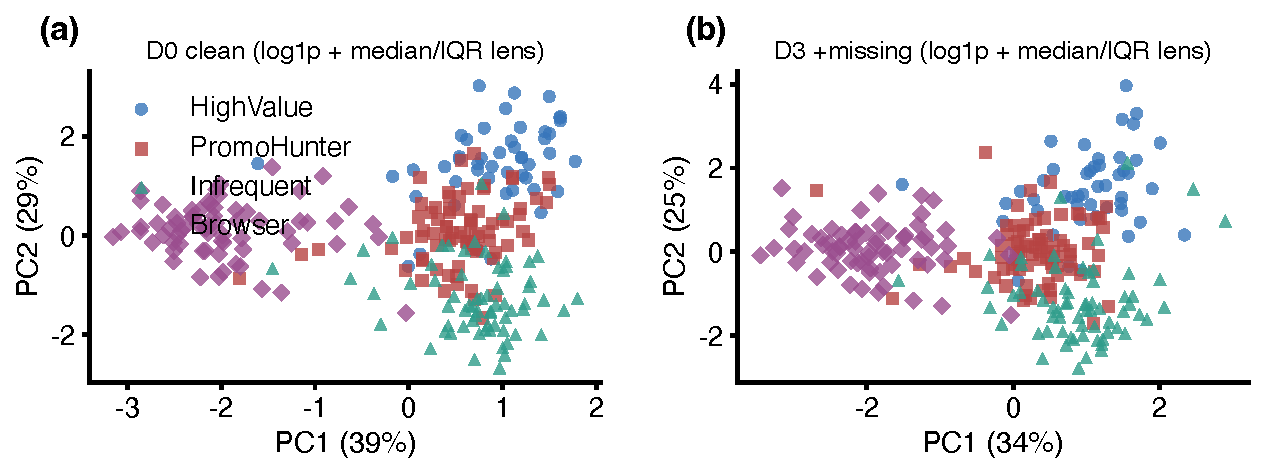
\includegraphics[width=\linewidth]{fig17_pca_hidden_segments.pdf}
\caption{Cấu trúc phân khúc ẩn trên không gian PCA 2 chiều (cùng cách biểu diễn log1p, median/IQR; chỉ để chẩn đoán). (a) Dữ liệu sạch D0: bốn nhóm tách được nhưng chồng lấn do khách ``cầu nối''.
(b) D3 sau khi thêm nhiễu, ngoại lai và giá trị thiếu: cấu trúc bị méo và các nhóm trộn nhiều hơn.}
\label{fig:a_pca}
\end{figure}

\subsection{Giả định của cơ chế sinh}
\begin{itemize}
\item Bốn đặc điểm ẩn, các phương trình và mọi hệ số do chúng tôi đặt, không rút từ dữ liệu thật; không mô hình hóa thời gian hay mùa vụ; mỗi khách có ít nhất một đơn trong năm.
\item Nhiễu độc lập giữa các cột; cơ chế thiếu MCAR/MAR được giả định, không suy ra từ dữ liệu thật.
\item Một sai khác so với thiết kế đã thống nhất: bỏ phụ thuộc ``mức dùng khuyến mãi giảm theo hạng gold'' vì tạo vòng lặp (hạng suy từ tổng chi, tổng chi suy từ khuyến mãi).
\end{itemize}
\FloatBarrier

\section{Hiểu dữ liệu (Data Understanding)}
\label{sec:b}

Phần A của bước này (``mù'') chỉ đọc D3 và data dictionary: tổng quan, thống kê mô tả, phân phối, giá trị thiếu, tương quan, ngoại lai bằng sáu phương pháp và phân tích khoảng cách/mật độ. Phần B mới đọc D0--D2 và nhật ký chèn lỗi,
để đo tác động từng thao tác và kiểm chứng các phát hiện mù.

\subsection{Tổng quan và phân phối}
D3 có 260 dòng $\times$ 14 thuộc tính (cùng \var{customer_id} duy nhất, không dòng trùng). Khoảng giá trị thực tế \emph{vượt miền khai báo} ở nhiều cột (tuổi tới 150, thời lượng phiên 1440 phút, số phiên 999).
Mười cột số đều lệch phải ở mức khác nhau (Bảng~\ref{tab:desc}); 80 khách (30,8\%) chỉ có đúng 1 đơn và 11 khách chạm trần recency 365 ngày.

\begin{table}[htbp]
\centering\small
\caption{Thống kê mô tả của D3 (chưa xử lý). Tỉ số $s/s_{\mathrm{bền}}$ là độ lệch chuẩn chia độ lệch chuẩn bền (IQR/1,349): lớn nghĩa là vài giá trị cực trị làm phồng độ lệch chuẩn.}
\label{tab:desc}
\begin{tabular}{lrrrrrr}
\toprule
Thuộc tính & Trung vị & Trung bình & Skew & $s/s_{\mathrm{bền}}$ & Lớn nhất\\
\midrule
\var{age} & 32 & 33,6 & 3,33 & 1,15 & 150\\
\var{n_orders_12m} & 5 & 15,5 & 3,33 & 1,93 & 178\\
\var{avg_order_value} & 43,8 & 86,9 & 9,19 & 10,62 & 3\,093\\
\var{total_spend_12m} & 211,7 & 1\,455 & 8,52 & 9,33 & 62\,272\\
\var{recency_days} & 42 & 81,3 & 1,69 & 1,53 & 365\\
\var{discount_usage_rate} & 0,21 & 0,39 & 0,83 & 0,65 & 1,80\\
\var{sessions_per_month} & 10,05 & 14,9 & 15,70 & 7,67 & 999\\
\var{avg_session_minutes} & 8,5 & 18,9 & 14,84 & 11,14 & 1\,440\\
\var{pages_per_session} & 7,2 & 10,5 & 1,64 & 1,40 & 46,7\\
\var{cart_abandon_rate} & 0,42 & 0,52 & 0,74 & 0,83 & 1,35\\
\bottomrule
\end{tabular}
\end{table}

\subsection{Giá trị thiếu}
Ba cột có giá trị thiếu: \var{age} 21 ô (8,1\%), \var{avg_session_minutes} 31 ô (11,9\%), \var{preferred_category} 13 ô (5,0\%). Tổng cộng 61/260 dòng (23,5\%) có ít nhất một ô thiếu, nên xóa dòng sẽ mất gần một phần tư dữ liệu.
Tỉ lệ thiếu của \var{avg_session_minutes} khác nhau theo thiết bị (desktop 21,8\%, tablet 12,2\%, mobile 6,4\%); kiểm định hoán vị cho $p = 0{,}0037$ \emph{nhưng sau hiệu chỉnh Bonferroni cho 39 phép thử là $p = 0{,}144$}, nghĩa là
dấu hiệu MAR có nhưng chưa vượt được đa phép thử. Với \var{preferred_category}, kiểm định $\chi^2$ cho $p = 0{,}0006$ nhưng số kỳ vọng nhỏ nhất chỉ 2,05 ($<5$) nên xấp xỉ không đáng tin; kiểm định hoán vị cho $p = 0{,}0015$, Bonferroni $0{,}0585$, tức chưa đủ bằng chứng.

\begin{figure}[htbp]
\centering
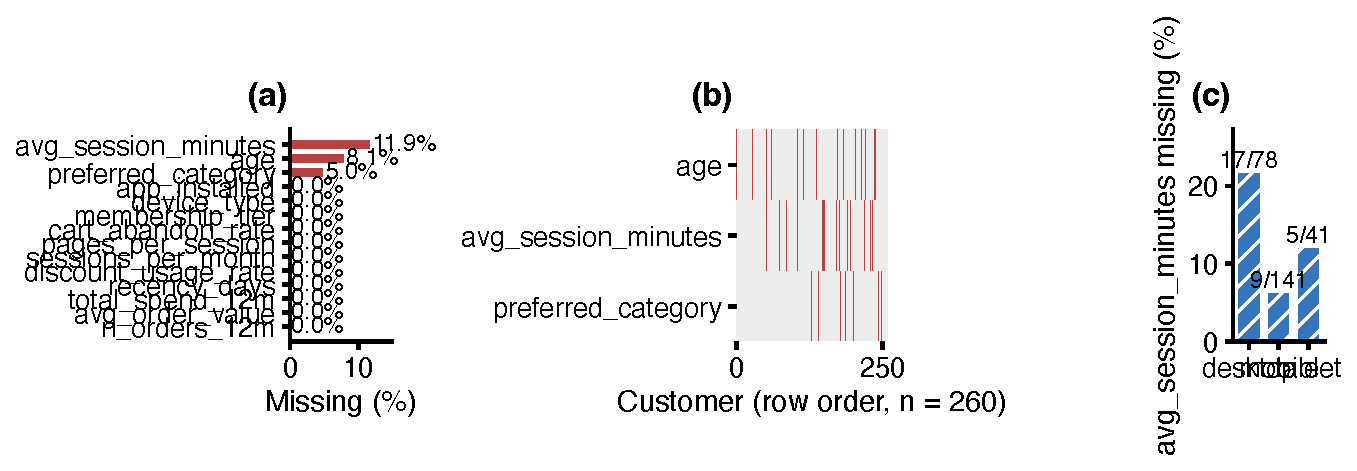
\includegraphics[width=\linewidth]{fig02_missing_values.pdf}
\caption{Giá trị thiếu trong D3. (a) Tỉ lệ thiếu theo cột. (b) Vị trí ô thiếu theo từng khách: không có mẫu thiếu theo khối. (c) Tỉ lệ thiếu của \var{avg_session_minutes} theo thiết bị.}
\label{fig:b_missing}
\end{figure}

\subsection{Quan hệ giữa các thuộc tính}
Tương quan hạng Spearman cho thấy các cặp mạnh: \var{n_orders_12m} $\sim$ \var{total_spend_12m} ($0{,}92$), \var{avg_session_minutes} $\sim$ \var{pages_per_session} ($0{,}85$),
\var{n_orders_12m} $\sim$ \var{recency_days} ($-0{,}75$), \var{sessions_per_month} $\sim$ \var{pages_per_session} ($0{,}74$). Hệ số VIF trên hạng của \var{total_spend_12m} và \var{n_orders_12m} đều xấp xỉ 23; ma trận tương quan cần 3 thành phần để giữ 80\% và 5 thành phần để giữ 90\% phương sai (trên 10 biến số),
nghĩa là số chiều hiệu dụng chỉ bằng khoảng một nửa số cột.
Điểm đáng chú ý nhất là \textbf{Pearson thô và Spearman lệch nhau rất nhiều} do các ô hỏng: tương quan giữa thời lượng phiên và số trang là $0{,}049$ theo Pearson nhưng $0{,}848$ theo Spearman (Hình~\ref{fig:b_corr}).
Ở dữ liệu sạch, cùng cặp này có Pearson $0{,}906$: ô hỏng đã phá hủy quan hệ tuyến tính.

\begin{figure}[htbp]
\centering
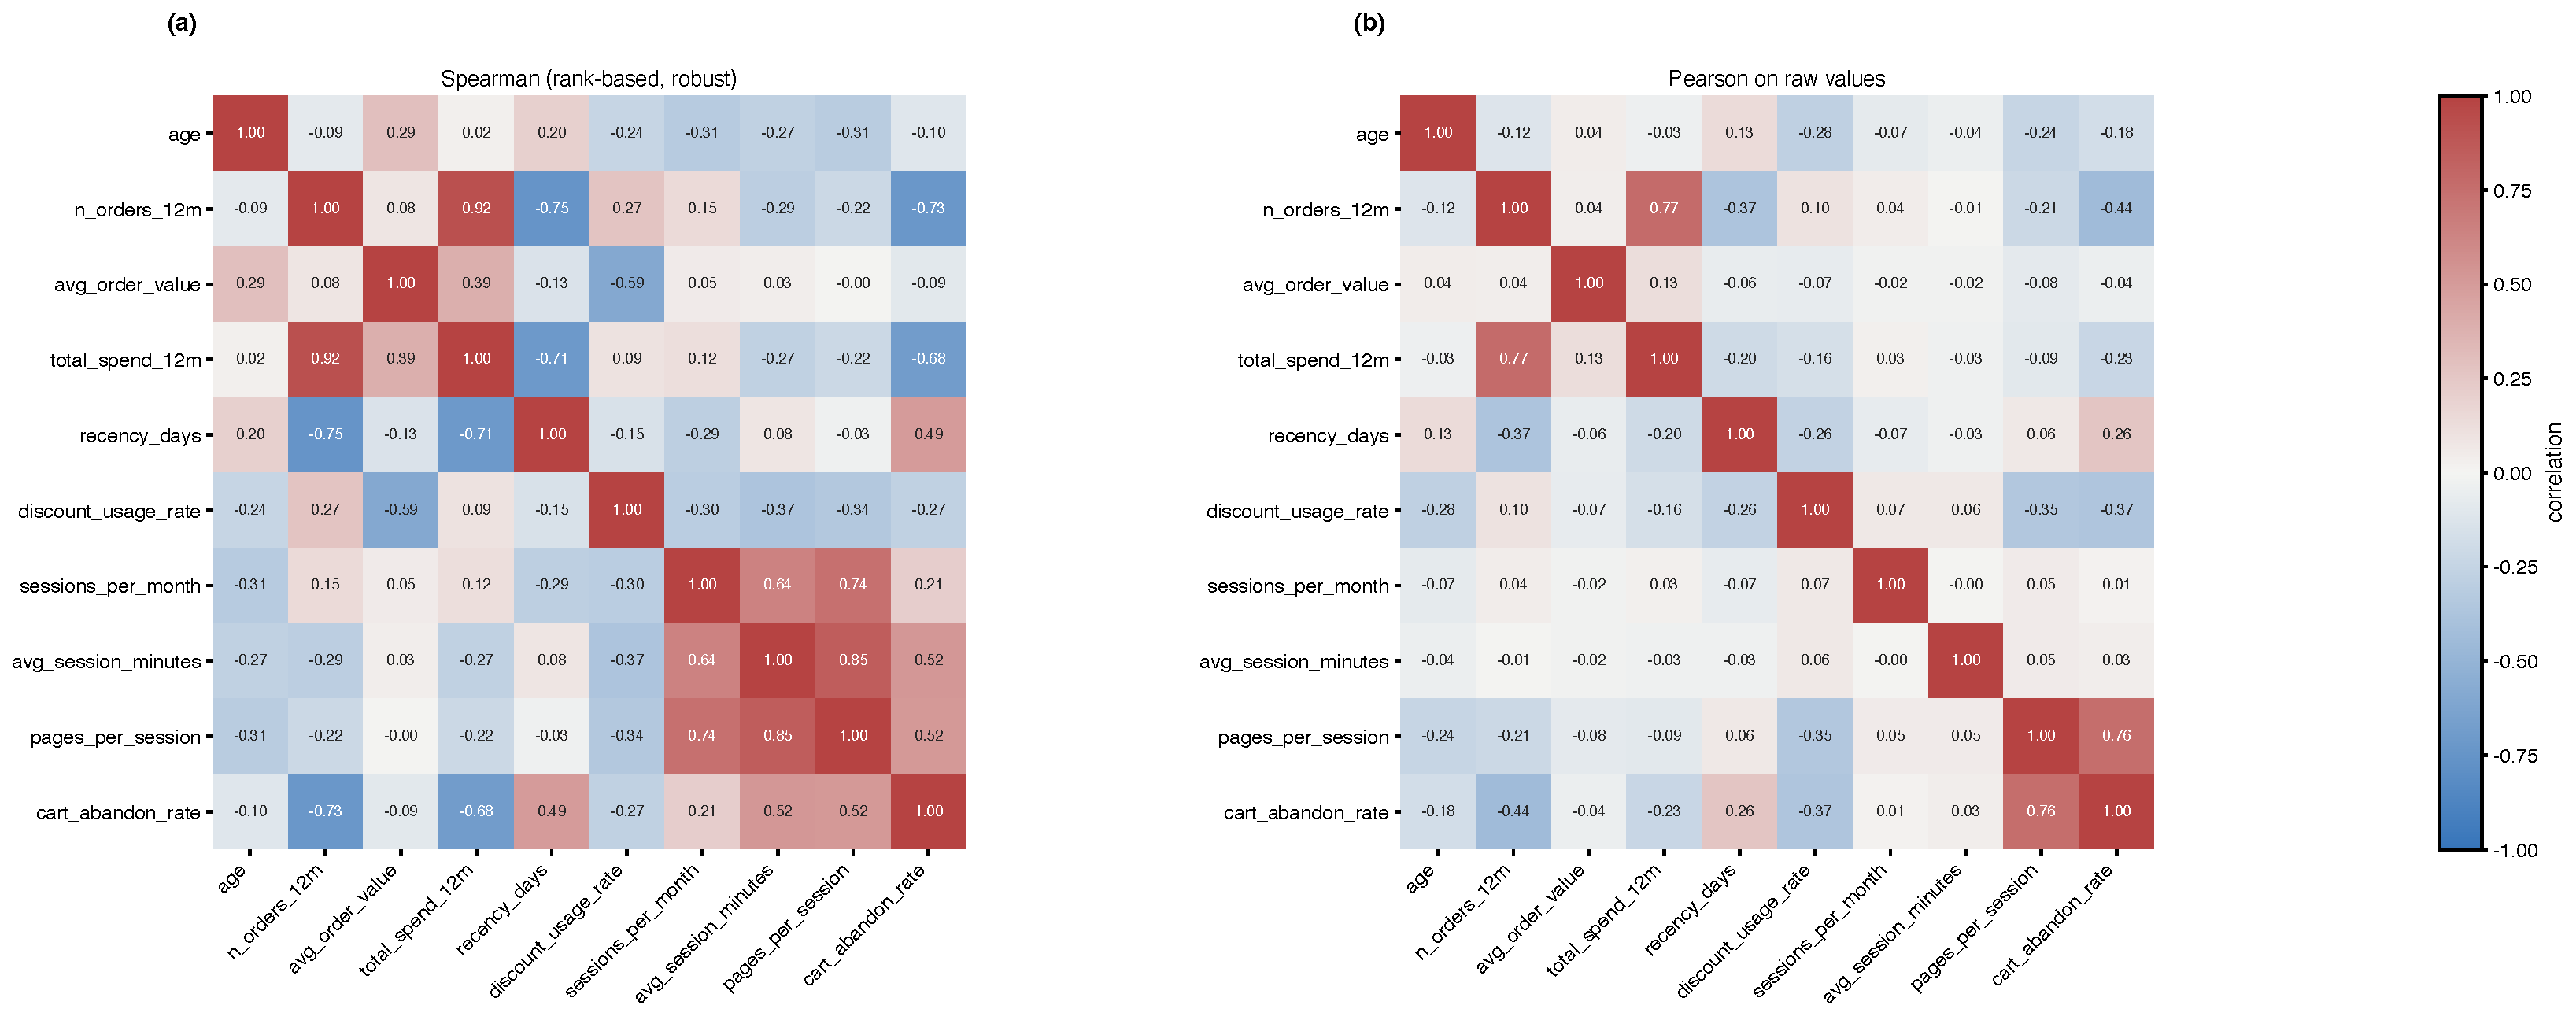
\includegraphics[width=\linewidth]{fig08_correlation_numeric.pdf}
\caption{Ma trận tương quan 10 biến số của D3: (a) Spearman (dựa hạng, bền); (b) Pearson trên giá trị thô. Các cặp có liên quan tới \var{sessions_per_month} và \var{avg_session_minutes} gần như mất tương quan ở (b).}
\label{fig:b_corr}
\end{figure}

\subsection{Giá trị bất thường}
Sáu phương pháp cho kết quả rất khác nhau (Bảng~\ref{tab:outlier}). Luật miền nghiệp vụ cộng với kiểm tra đẳng thức xấp xỉ $\mathrm{total}\approx\mathrm{n\_orders}\times\mathrm{AOV}$ gắn cờ đúng 7 dòng lỗi,
trong khi Tukey $1{,}5$ IQR gắn cờ 94 dòng (36,2\%) chỉ vì phân phối lệch phải. Sau khi đối chiếu với nhật ký (Phần B), độ chính xác (precision) của Tukey $1{,}5$ chỉ là $0{,}14$, và phương pháp thống kê chung gắn cờ cả 8 khách cực trị \emph{hợp lệ}
cùng hàng chục dòng bình thường. Do đó không thể dùng một ngưỡng thống kê để xóa ngoại lai.

\begin{table}[htbp]
\centering\small
\caption{Phát hiện ngoại lai ở Phần A (mù) và kiểm chứng ở Phần B với 15 khách thực sự bị chèn (8 hợp lệ, 7 lỗi).}
\label{tab:outlier}
\begin{tabular}{lrrrrr}
\toprule
Phương pháp & Số dòng gắn cờ & Bắt được & Precision & Recall lỗi (7) & Recall hợp lệ (8)\\
\midrule
Luật miền + đẳng thức & 7 & 7 & 1,00 & 7/7 & 0/8\\
Tukey $1{,}5$ IQR & 94 & 13 & 0,14 & 5/7 & 8/8\\
Tukey $3$ IQR & 38 & 12 & 0,32 & 4/7 & 8/8\\
Robust $z>3{,}5$ (trên log) & 33 & 10 & 0,30 & 6/7 & 4/8\\
LOF ($k=20$) & 10 & 9 & 0,90 & 6/7 & 3/8\\
\bottomrule
\end{tabular}
\end{table}

\subsection{Các vấn đề dữ liệu chính và tác động đo được lên khoảng cách, mật độ và cấu trúc cụm}
Vì phân cụm dựa vào khoảng cách, phần quan trọng nhất là xem các vấn đề dữ liệu làm thay đổi hình học thế nào (Hình~\ref{fig:b_dist}, Bảng~\ref{tab:stages}):
\begin{itemize}
\item \textbf{Thang đo và ô hỏng quyết định khoảng cách.} Khi không chuẩn hóa, \var{total_spend_12m} chiếm 99,59\% tổng phương sai. Sau z-score thô, 7 dòng lỗi (2,7\% số dòng) vẫn chiếm 31,4\% tổng bình phương khoảng cách của mọi cặp;
một ô \var{sessions_per_month}=999 kéo độ lệch chuẩn cột này lên 61,8 so với 8,1 theo thang bền, nén 259 dòng còn lại về gần hằng số ở cột đó.
\item \textbf{Lân cận cục bộ rất nhạy.} Chỉ riêng nhiễu đã làm mất 21--33\% lân cận 5-NN dù phân phối biên gần như không đổi (thống kê KS $0{,}03$--$0{,}05$); thêm ngoại lai còn $0{,}53$--$0{,}62$ lân cận được giữ lại.
\item \textbf{Thống kê Hopkins bị phồng khi có ngoại lai} (từ $0{,}83$ lên $0{,}94$ với z-score thô) do khung dữ liệu bị kéo giãn, nên không đáng tin để kết luận ``dữ liệu có cụm'' trên D3.
\item \textbf{Phân phối lệch phải nặng với biên cứng.} Trung bình gấp $6{,}9$ lần trung vị với \var{total_spend_12m} và $3{,}1$ lần với \var{n_orders_12m}; 7/10 cột có độ lệch $>1$ sau khi loại các ô vi phạm miền; 80 khách (30,8\%) dồn ở đúng 1 đơn.
Hệ quả đo được: ngay cả sau z-score thô, 5 dòng lớn nhất vẫn nắm $21{,}9\%$ tổng bình phương độ lệch và $17$ ô vượt $4$ độ lệch chuẩn (Bảng~\ref{tab:scaler}); sau log1p con số này là $6{,}6\%$ và $2$ ô.
\item \textbf{Thông tin trùng lặp.} Số đơn và tổng chi có Spearman $0{,}92$ (VIF $\approx 23$); trên thang log, tổng chi được giải thích gần hết bởi số đơn và giá trị đơn ($R^2 = 0{,}987$); ma trận tương quan chỉ cần 3--5 thành phần cho 80--90\% phương sai.
Nghĩa là các trục này bị đếm nhiều lần trong khoảng cách.
\item \textbf{Giá trị thiếu ở 23,5\% số dòng.} Xóa dòng làm mất 61 khách; tỉ lệ thiếu của thời lượng phiên chênh theo thiết bị ($6{,}4\%$ đến $21{,}8\%$) nên xóa dòng còn làm lệch cơ cấu thiết bị.
\item \textbf{Độ tách phân khúc giảm}: Silhouette theo nhãn ẩn (chỉ chẩn đoán) giảm từ $0{,}327$ xuống $0{,}288$ trên biểu diễn log1p + median/IQR.
\end{itemize}

\begin{figure}[htbp]
\centering
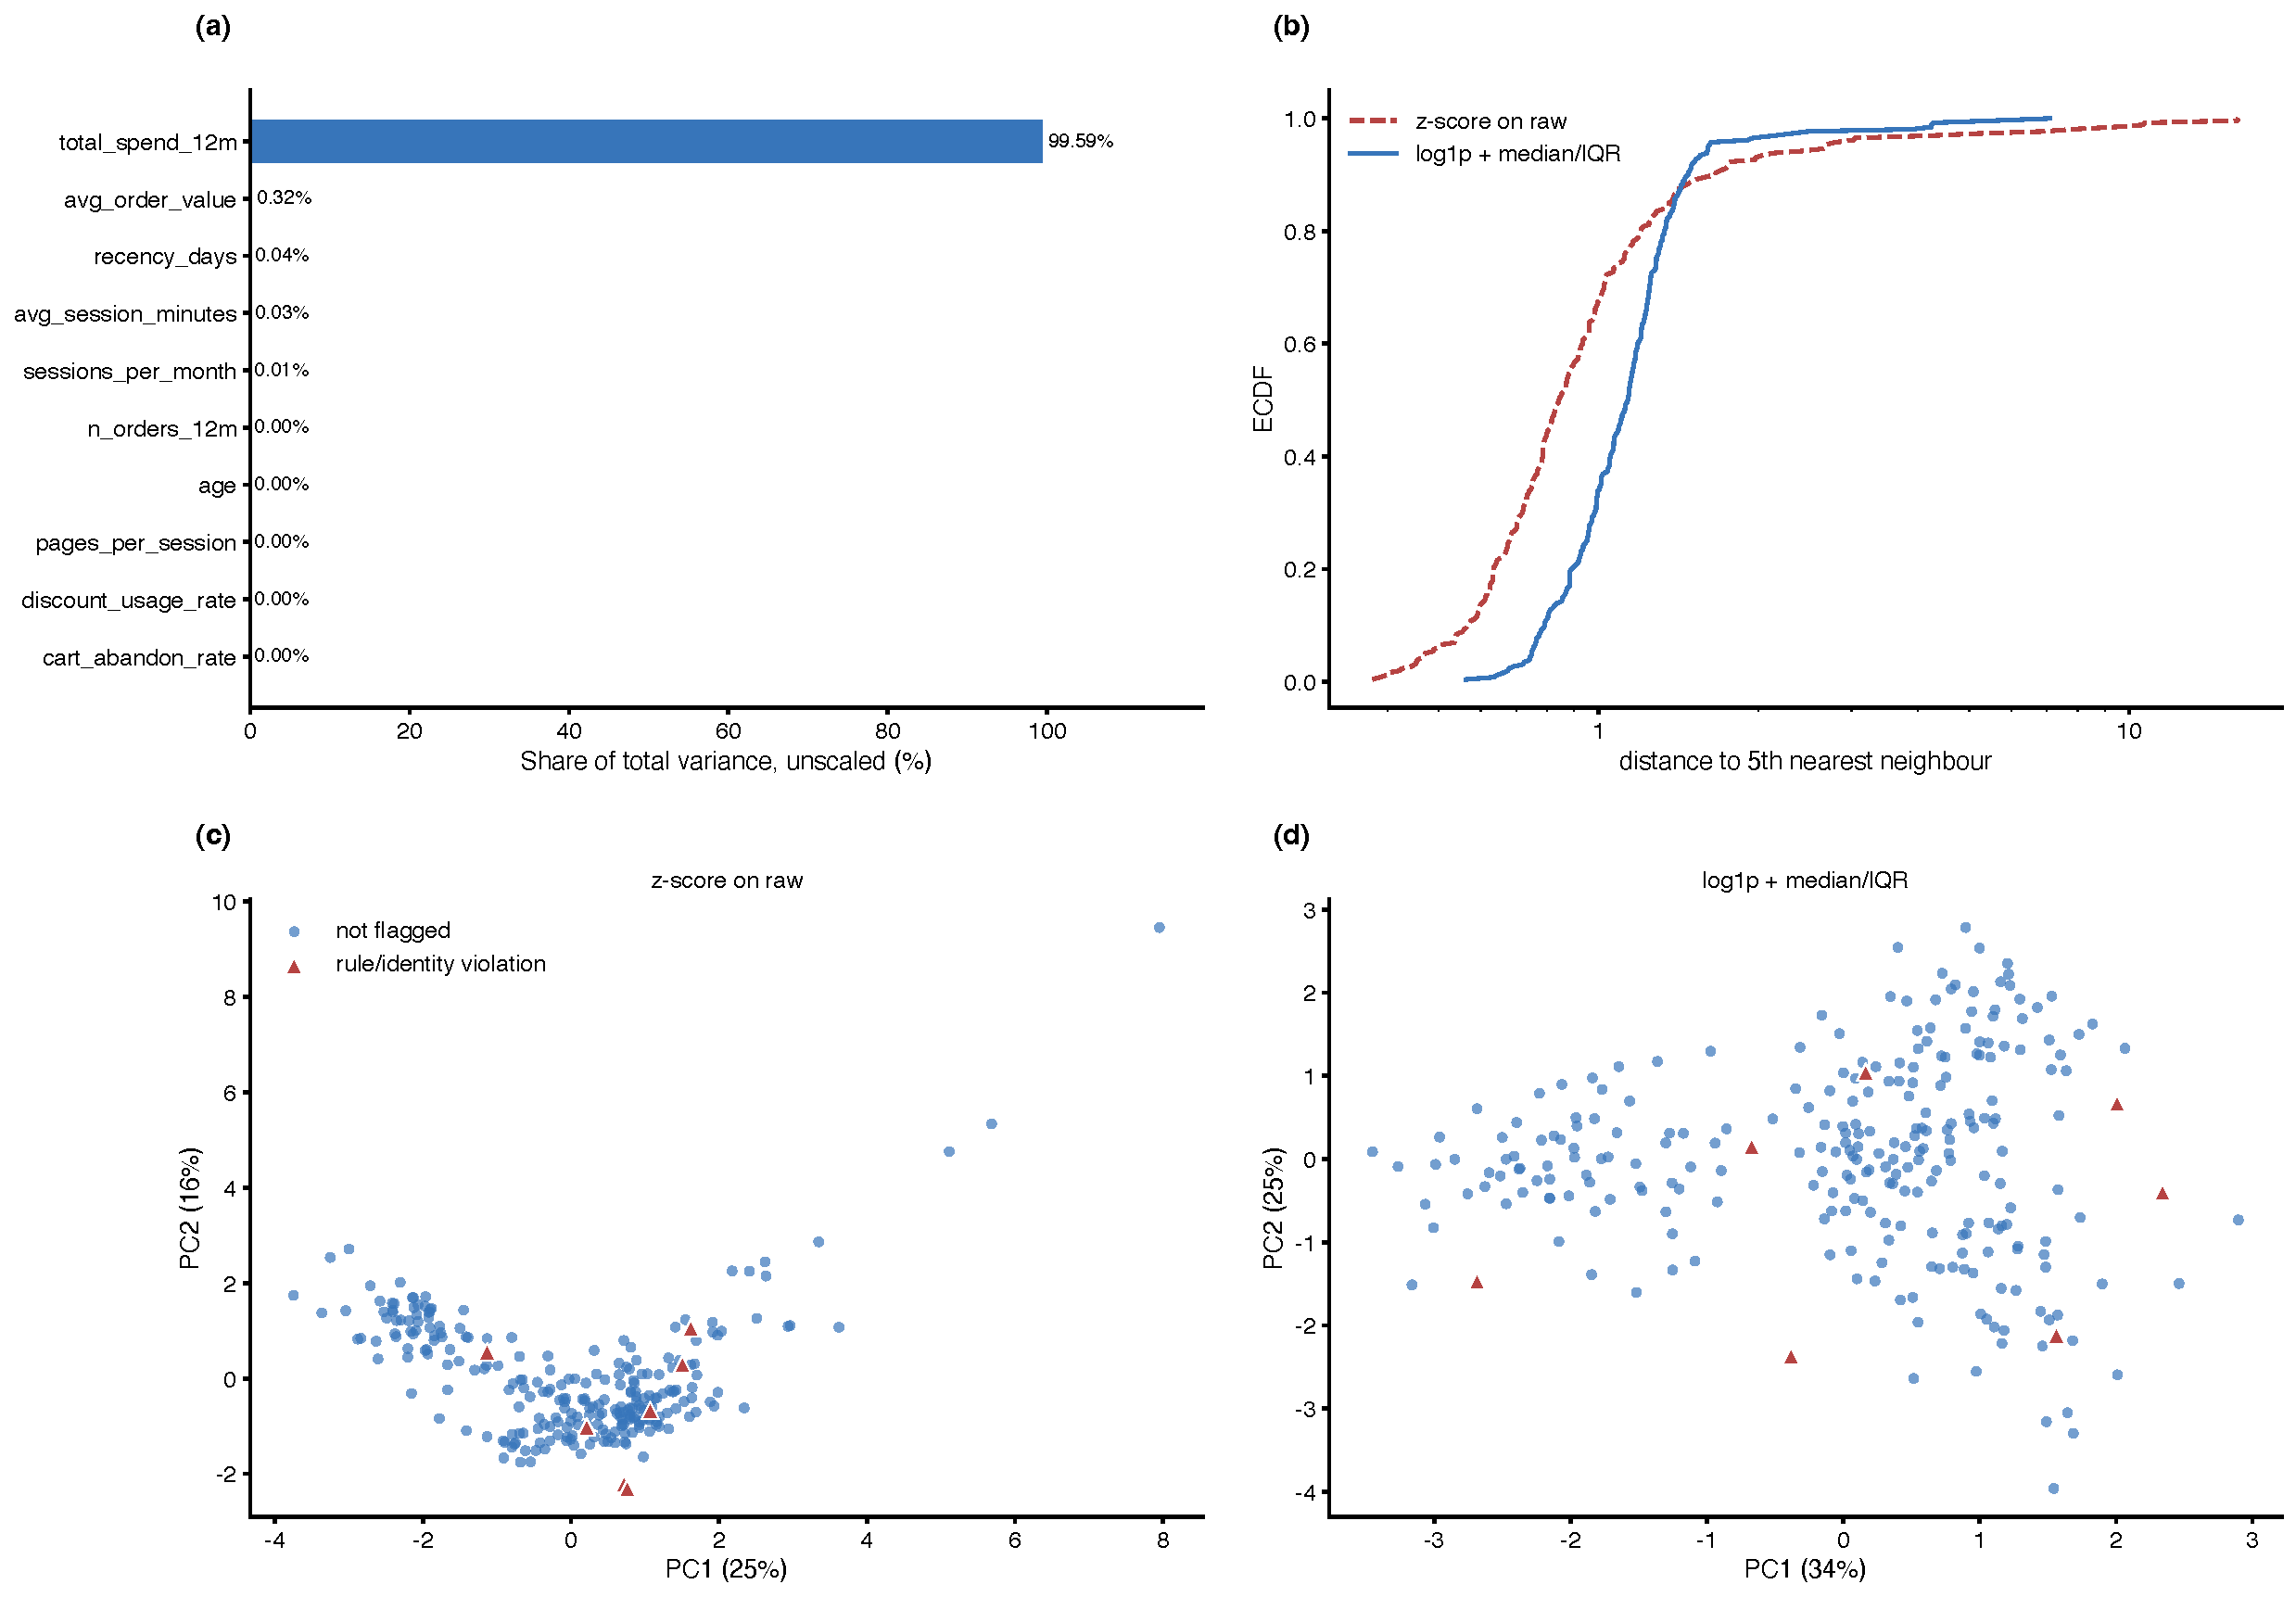
\includegraphics[width=0.92\linewidth]{fig12_distance_and_density.pdf}
\caption{Tác động lên khoảng cách và mật độ (D3). (a) Phần phương sai thô của từng thuộc tính: một cột chiếm 99,6\%. (b) ECDF khoảng cách tới láng giềng thứ 5: đuôi rất dài với z-score thô.
(c, d) Chiếu PCA 2 chiều: các dòng vi phạm luật miền/đẳng thức (tam giác) bị đẩy ra xa ở z-score thô, ít hơn ở log1p + median/IQR.}
\label{fig:b_dist}
\end{figure}

\begin{table}[htbp]
\centering\small
\caption{Cấu trúc qua bốn giai đoạn dữ liệu (so với D0). Mỗi ô: z-score thô / log1p + median/IQR.}
\label{tab:stages}
\begin{tabular}{lcccc}
\toprule
Giai đoạn & 5-NN giữ lại & Tương quan hạng khoảng cách & Hopkins & Silhouette (nhãn ẩn)\\
\midrule
D0 sạch & 1,00 / 1,00 & 1,00 / 1,00 & 0,833 / 0,724 & 0,298 / 0,327\\
D1 + nhiễu & 0,79 / 0,67 & 0,99 / 0,98 & 0,837 / 0,718 & 0,294 / 0,317\\
D2 + ngoại lai & 0,55 / 0,62 & 0,78 / 0,87 & 0,939 / 0,835 & 0,281 / 0,297\\
D3 + thiếu & 0,53 / 0,57 & 0,77 / 0,86 & 0,940 / 0,835 & 0,281 / 0,288\\
\bottomrule
\end{tabular}
\end{table}
\FloatBarrier

\section{Tiền xử lý dữ liệu (Data Preprocessing)}
\label{sec:c}

\subsection{Nguyên tắc và kiểm soát rò rỉ}
Phương án xử lý chỉ dựa trên các phát hiện của Phần A (chỉ đọc D3). Script \var{03_preprocess.py} chỉ có một lệnh đọc dữ liệu, nằm trong hàm kiểm tra đường dẫn chỉ cho phép D3 và data dictionary;
nghiệm thu còn quét mã nguồn để bảo đảm không chứa tên D0--D2 hay thư mục dữ liệu ẩn. Sau khi 15/15 kiểm tra nghiệm thu đạt, bốn file kết quả được ghi mã băm SHA-256 và khóa ghi;
script đối chiếu \var{03b_evaluate_preprocessing.py} từ chối chạy nếu mã băm lệch (đã thử: sửa 1 byte thì bị từ chối). Chỉ sau đó D0 mới được mở, và chỉ để tính số đo tổng hợp, \emph{không} dùng để thay thế từng giá trị.
Đầu ra giữ nguyên đơn vị và độ chính xác gốc; log, chuẩn hóa và mã hóa được thực hiện ở bước chuẩn bị dữ liệu (mục~\ref{sec:d}).

\subsection{Phương án xử lý và cơ sở}
\begin{table}[htbp]
\centering\small
\caption{Quyết định tiền xử lý. Mọi cơ sở lấy từ D3; mọi thay đổi ghi vào nhật ký từng ô (72 ô).}
\label{tab:cdecisions}
\begin{tabularx}{\linewidth}{>{\raggedright\arraybackslash}p{2.6cm}>{\raggedright\arraybackslash}X>{\raggedright\arraybackslash}X}
\toprule
Vấn đề & Quyết định & Cơ sở và phương án đã loại\\
\midrule
7 ô không hợp lệ & Giữ nguyên dòng; vô hiệu hóa \emph{từng ô} (6 vi phạm luật miền, 1 vi phạm đẳng thức) rồi điền. &
Mỗi dòng chỉ hỏng một ô, 13 ô còn lại hợp lệ. Loại: xóa dòng; cắt ngưỡng (tạo điểm dồn giả ở biên).\\
Dòng C0062 (AOV 3\,093 so với total$/n$ = 40,04) & Vô hiệu hóa ô AOV và điền bằng mô hình như mọi ô khác; \textbf{không} gán $\mathrm{AOV}=\mathrm{total}/n$. &
Data Dictionary ghi $\mathrm{total}\sim n\times\mathrm{AOV}$ (xấp xỉ), không xác nhận đẳng thức chính xác, và sd bền của độ lệch đẳng thức ở dòng bình thường là $0{,}164$ ($\approx 16\%$). Ô nghi chọn theo phân vị biên: AOV 99,6\%, total 60,8\%, $n$ 59,2\%; hạng bronze khớp với total thấp.\\
Giá trị thiếu (số) & Chọn phương pháp điền theo thí nghiệm che ô (Bảng~\ref{tab:imp}). & Trung vị toàn cục tạo 22--32 giá trị trùng; xóa dòng mất 23,5\%.\\
\var{preferred_category} & Giữ mức \texttt{unknown}; các biến thể KNN-7/mode được lưu riêng để so sánh (Bảng~\ref{tab:sens}). &
Độ chính xác che ô tốt nhất $0{,}40$ nên nhãn điền vào sai nhiều hơn đúng (mục~\ref{sec:c_cat}).\\
Nhiễu & \textbf{Không khử nhiễu từng giá trị}; không làm mượt, không winsorize. &
Nhiễu độc lập từng ô không phục hồi được từ D3; làm mượt trộn khách khác nhóm và co các hồ sơ hiếm; winsorize tạo điểm dồn.\\
Cực trị hợp lệ & Chỉ ghi cờ (34 dòng, 56 ô ngoài 3 IQR và không vi phạm luật nào), không sửa, không xóa. &
Tukey $1{,}5$ IQR gắn cờ 94 dòng với precision $0{,}14$; xóa sẽ loại nhóm khách giá trị cao thật.\\
Điểm dồn ở biên & Giữ nguyên, ghi cờ; không ô nào được điền rơi đúng giá trị biên. &
Thấy ngay trong D3: \var{sessions_per_month}=0,5 (12 dòng), \var{recency_days}=0 (15), =365 (11), \var{n_orders_12m}=1 (80), \var{age}=18 (22). Jitter là bịa dữ liệu.\\
\bottomrule
\end{tabularx}
\end{table}

\subsection{Chọn phương pháp điền khuyết}
Với mỗi cột cần điền, 15\% ô \emph{đã quan sát} bị che ngẫu nhiên, lặp 50 lần với \textbf{cùng một tập mask cho mọi phương pháp} (so sánh ghép cặp); năm phương pháp được đo bằng MAE ở đơn vị gốc. Quy tắc 1-SE: chọn phương pháp \emph{đơn giản nhất}
(thứ tự trung vị $<$ trung vị theo thiết bị $<$ KNN5 $<$ KNN10 $<$ hồi quy lặp) có MAE không vượt MAE tốt nhất cộng một sai số chuẩn của nó. Với \var{age} sai số được báo bằng năm.

\begin{table}[htbp]
\centering\small
\caption{Thí nghiệm che ô: MAE trung bình (độ lệch chuẩn qua 50 lần; sai số chuẩn SE). In đậm là phương pháp được chọn.}
\label{tab:imp}
\begin{tabular}{lcc}
\toprule
Phương pháp & \var{age} (năm; 36 ô/lần) & \var{avg_session_minutes} (phút; 34 ô/lần)\\
\midrule
Trung vị toàn cục & 8,82 (0,84; SE 0,118) & 7,69 (1,41; SE 0,200)\\
Trung vị theo thiết bị & 8,13 (0,82; SE 0,116) & 7,65 (1,42; SE 0,200)\\
KNN ($k=5$) & 7,10 (0,89; SE 0,126) & 4,10 (0,95; SE 0,134)\\
KNN ($k=10$) & \textbf{6,89 (0,86; SE 0,122)} & 4,01 (0,93; SE 0,132)\\
Hồi quy lặp & 7,20 (0,79; SE 0,111) & \textbf{3,04 (0,60; SE 0,085)}\\
\bottomrule
\end{tabular}
\end{table}

Các cột còn lại (mỗi cột chỉ 1 ô cần điền) được chọn theo cùng quy tắc: \var{avg_order_value} và \var{recency_days} dùng hồi quy lặp; \var{discount_usage_rate} và \var{cart_abandon_rate} dùng KNN5;
\var{sessions_per_month} dùng KNN10. Tuổi gần như không đoán được từ các cột khác: KNN10 chỉ giảm MAE khoảng 22\% so với trung vị, nên các ô tuổi điền vào mang rất ít thông tin.

\subsubsection{Vì sao giữ \texttt{unknown} cho \var{preferred_category}}
\label{sec:c_cat}
Quyết định dựa trên mức bất định, không dùng một ngưỡng độ chính xác chung. Che 15\% ô, 50 lần, cùng mask: mode toàn cục đúng $0{,}254$, mode theo thiết bị $0{,}218$, mode theo hạng $0{,}197$, KNN-7 $0{,}402$.
KNN-7 hơn mode toàn cục $0{,}148$ (SE ghép cặp $0{,}013$): tốt hơn thật nhưng vẫn sai khoảng 60\% lần. Trên chính 13 ô thiếu, xác suất lớp dự đoán trung bình chỉ $0{,}53$ (từ $0{,}40$ đến $0{,}71$) và entropy chuẩn hóa $0{,}64$;
kỳ vọng sai khoảng $7{,}8$ trên 13 nhãn nếu điền. Một nhãn gán vào mà xác suất sai lớn hơn xác suất đúng, trên một biến chiếm 5\% dòng, là thông tin bịa thêm; \texttt{unknown} không bịa. Phân tích độ nhạy ở mục~\ref{sec:e} (Bảng~\ref{tab:sens}) cho thấy cách xử lý này không làm thay đổi đáng kể kết quả phân cụm.

\subsection{Kết quả xử lý (chỉ dựa trên D3 và dữ liệu đã xử lý)}
Có 72 ô thay đổi: 7 ô không hợp lệ được điền, 21 ô \var{age} và 31 ô \var{avg_session_minutes} thiếu được điền, 13 ô \var{preferred_category} thành \texttt{unknown}; mọi ô khác giữ nguyên từng giá trị.
Ô AOV của C0062 được điền $40{,}75$, gần total$/n=40{,}04$ (chỉ dùng kiểm tra hợp lý). Trên D3, phần bình phương khoảng cách do 7 dòng đã sửa gây ra giảm từ $0{,}314$ xuống $0{,}041$ (z-score thô) và từ $0{,}152$ xuống $0{,}044$ (log1p + median/IQR) (Hình~\ref{fig:c_struct});
độ lệch chuẩn của \var{sessions_per_month} so với độ lệch chuẩn bền giảm từ $7{,}7$ xuống $1{,}0$, của \var{avg_session_minutes} từ $11{,}1$ xuống $1{,}4$. Điểm dồn ở biên không đổi (12, 15, 11, 80, 22) và không ô điền nào rơi đúng giá trị biên.

\begin{figure}[htbp]
\centering
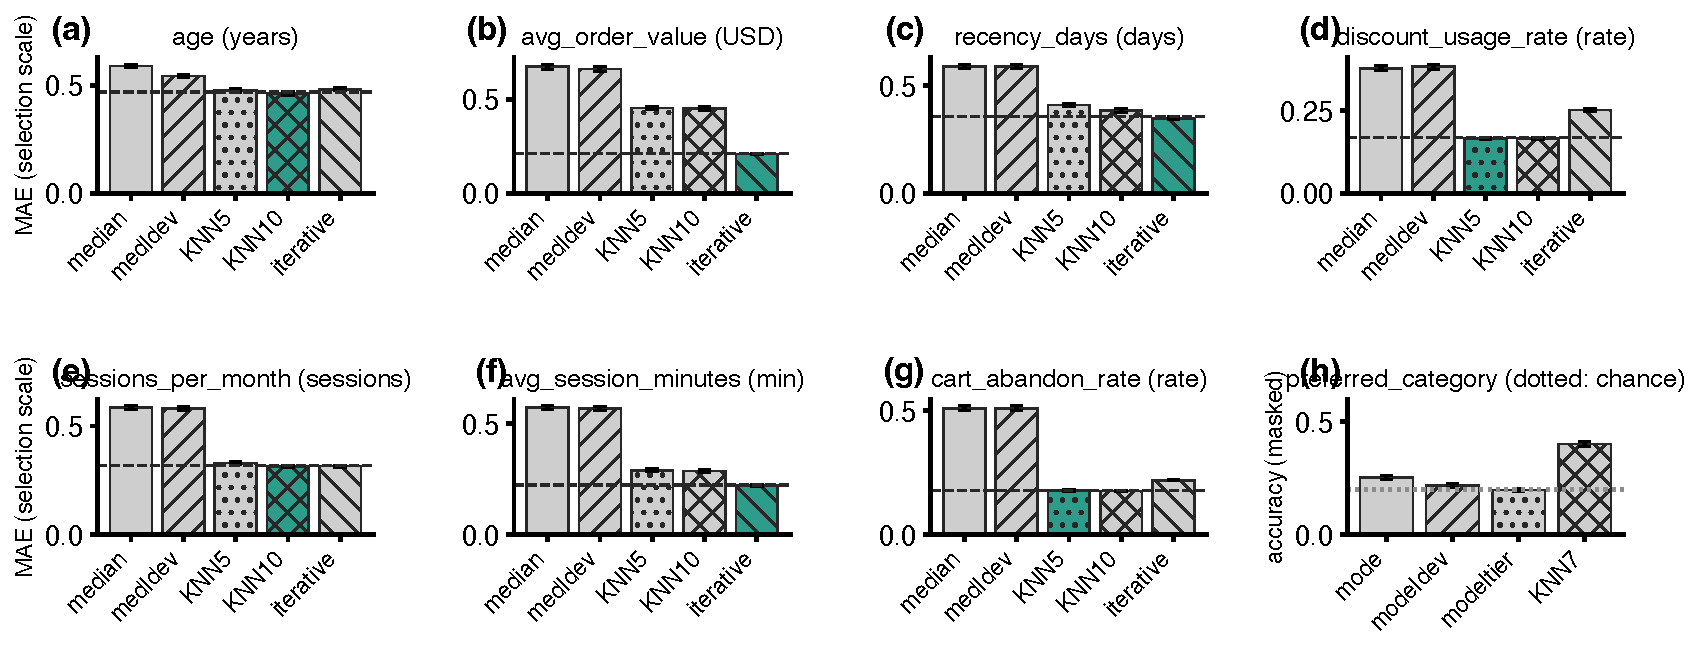
\includegraphics[width=\linewidth]{fig01_imputer_selection.pdf}
\caption{Chọn phương pháp điền: MAE (thang chọn, thanh sai số = SE; số ghi trên cột là MAE theo đơn vị gốc) cho từng cột và độ chính xác che ô của \var{preferred_category} (h).
Màu lam-lục là phương pháp được chọn; đường nét đứt là ngưỡng 1-SE.}
\label{fig:c_select}
\end{figure}

\begin{figure}[htbp]
\centering
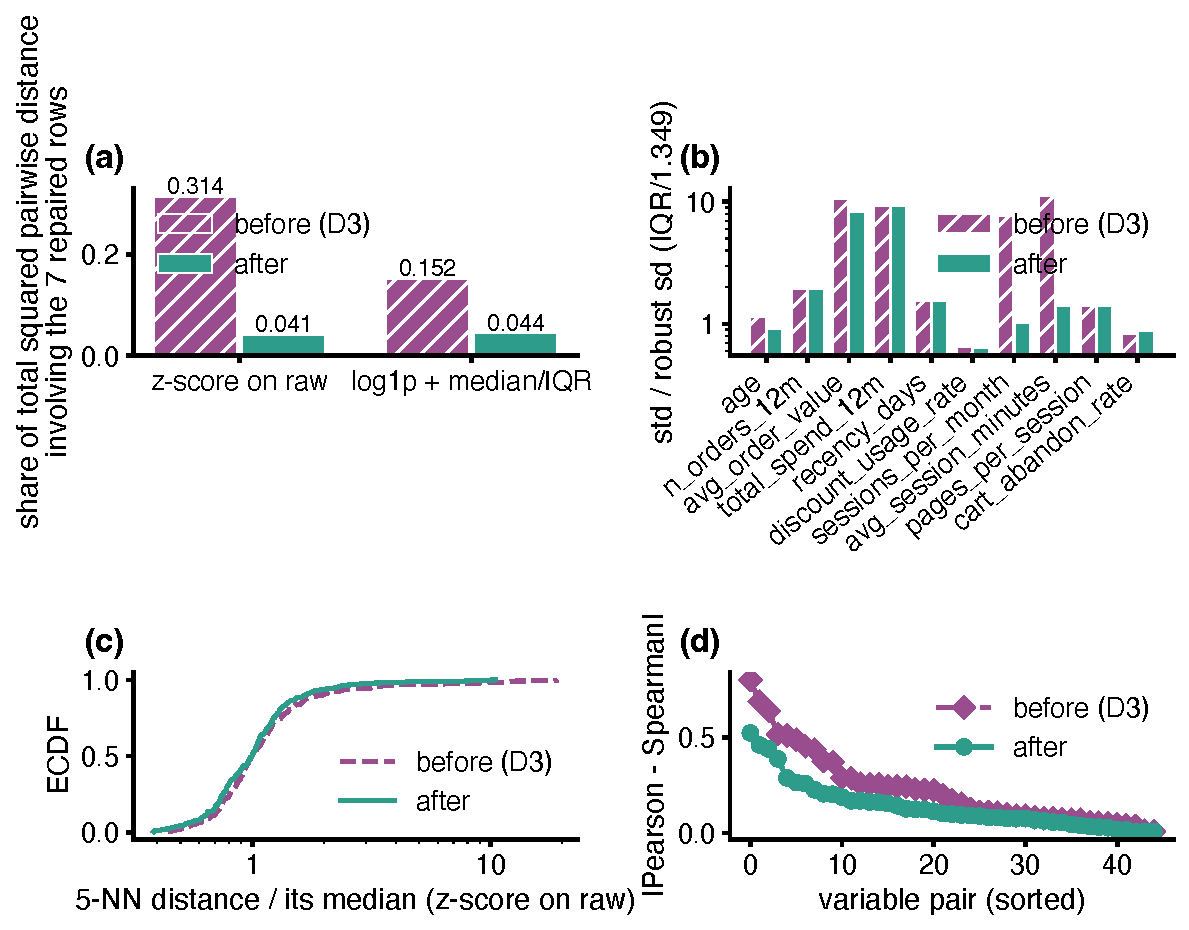
\includegraphics[width=0.92\linewidth]{fig04_structure_before_after.pdf}
\caption{Cấu trúc trước (D3) và sau xử lý, tính chỉ từ D3 và dữ liệu đã xử lý. (a) Phần bình phương khoảng cách liên quan 7 dòng đã sửa. (b) Độ lệch chuẩn chia độ lệch chuẩn bền theo cột.
(c) ECDF khoảng cách láng giềng thứ 5 chuẩn hóa theo trung vị. (d) Chênh lệch $|\text{Pearson}-\text{Spearman}|$ của các cặp biến.}
\label{fig:c_struct}
\end{figure}

\subsection{Đối chiếu với dữ liệu sạch (sau đóng băng)}
Các số đo dưới đây chỉ mô tả mức khớp tổng hợp với D0; chúng \emph{không} phải sai số khôi phục từng ô và không được dùng để chỉnh quy trình.
\begin{table}[htbp]
\centering\small
\caption{Mức khớp cấu trúc với D0 (z-score thô). Trước = D3; Sau = dữ liệu đã xử lý.}
\label{tab:c_eval}
\begin{tabular}{lccc}
\toprule
Số đo & D0 (tham chiếu) & Trước & Sau\\
\midrule
Trung bình $|\Delta$ Pearson$|$ so với D0 & 0 & 0,178 & 0,063\\
Trung bình $|\Delta$ Spearman$|$ so với D0 & 0 & 0,020 & 0,017\\
5-NN giữ lại so với D0 & 1,00 & 0,527 & 0,630\\
Tương quan hạng khoảng cách so với D0 & 1,00 & 0,772 & 0,878\\
Hopkins & 0,833 & 0,940 & 0,885\\
Silhouette theo nhãn ẩn (chẩn đoán) & 0,298 & 0,281 & 0,288\\
\bottomrule
\end{tabular}
\end{table}
\begin{itemize}
\item \textbf{Cải thiện rõ:} tỉ số độ lệch chuẩn với D0 của \var{sessions_per_month} giảm từ $8{,}31$ xuống $1{,}10$, của \var{avg_session_minutes} từ $9{,}07$ xuống $1{,}03$; sai khác Pearson với D0 giảm từ $0{,}178$ xuống $0{,}063$.
Với 31 ô \var{avg_session_minutes} được điền, MAE so với D0 là $2{,}95$ phút (mốc trung vị toàn cục $6{,}23$; sàn nhiễu $|\mathrm{D2}-\mathrm{D0}|$ là $2{,}15$); tương quan với D0 là $0{,}92$.
\item \textbf{Cải thiện khiêm tốn:} 21 ô \var{age} có MAE $7{,}14$ năm (mốc $8{,}24$), tương quan $0{,}58$, và độ phân tán chỉ bằng $0{,}53$ lần giá trị thật (điền đơn trị co phương sai).
\item \textbf{Không cải thiện hoặc xấu đi:} thống kê KS của \var{age} tăng từ $0{,}011$ lên $0{,}023$; KS của \var{sessions_per_month} giữ $0{,}050$ (do điểm dồn ở $0{,}5$); độ lệch của \var{avg_order_value} tăng từ $9{,}19$ lên $10{,}92$
vì các giá trị cực trị hợp lệ còn nguyên; số đo 5-NN chỉ đạt $0{,}63$ vì nhiễu chưa được xử lý.
\item \textbf{Một lần điền sai nhiều:} ô \var{recency_days} của C0242 được điền 210 ngày trong khi D0 là 69 (mốc trung vị toàn cục 26). Tôi không đổi phương pháp sau khi biết kết quả này để tránh rò rỉ từ dữ liệu sạch.
\end{itemize}

\begin{figure}[htbp]
\centering
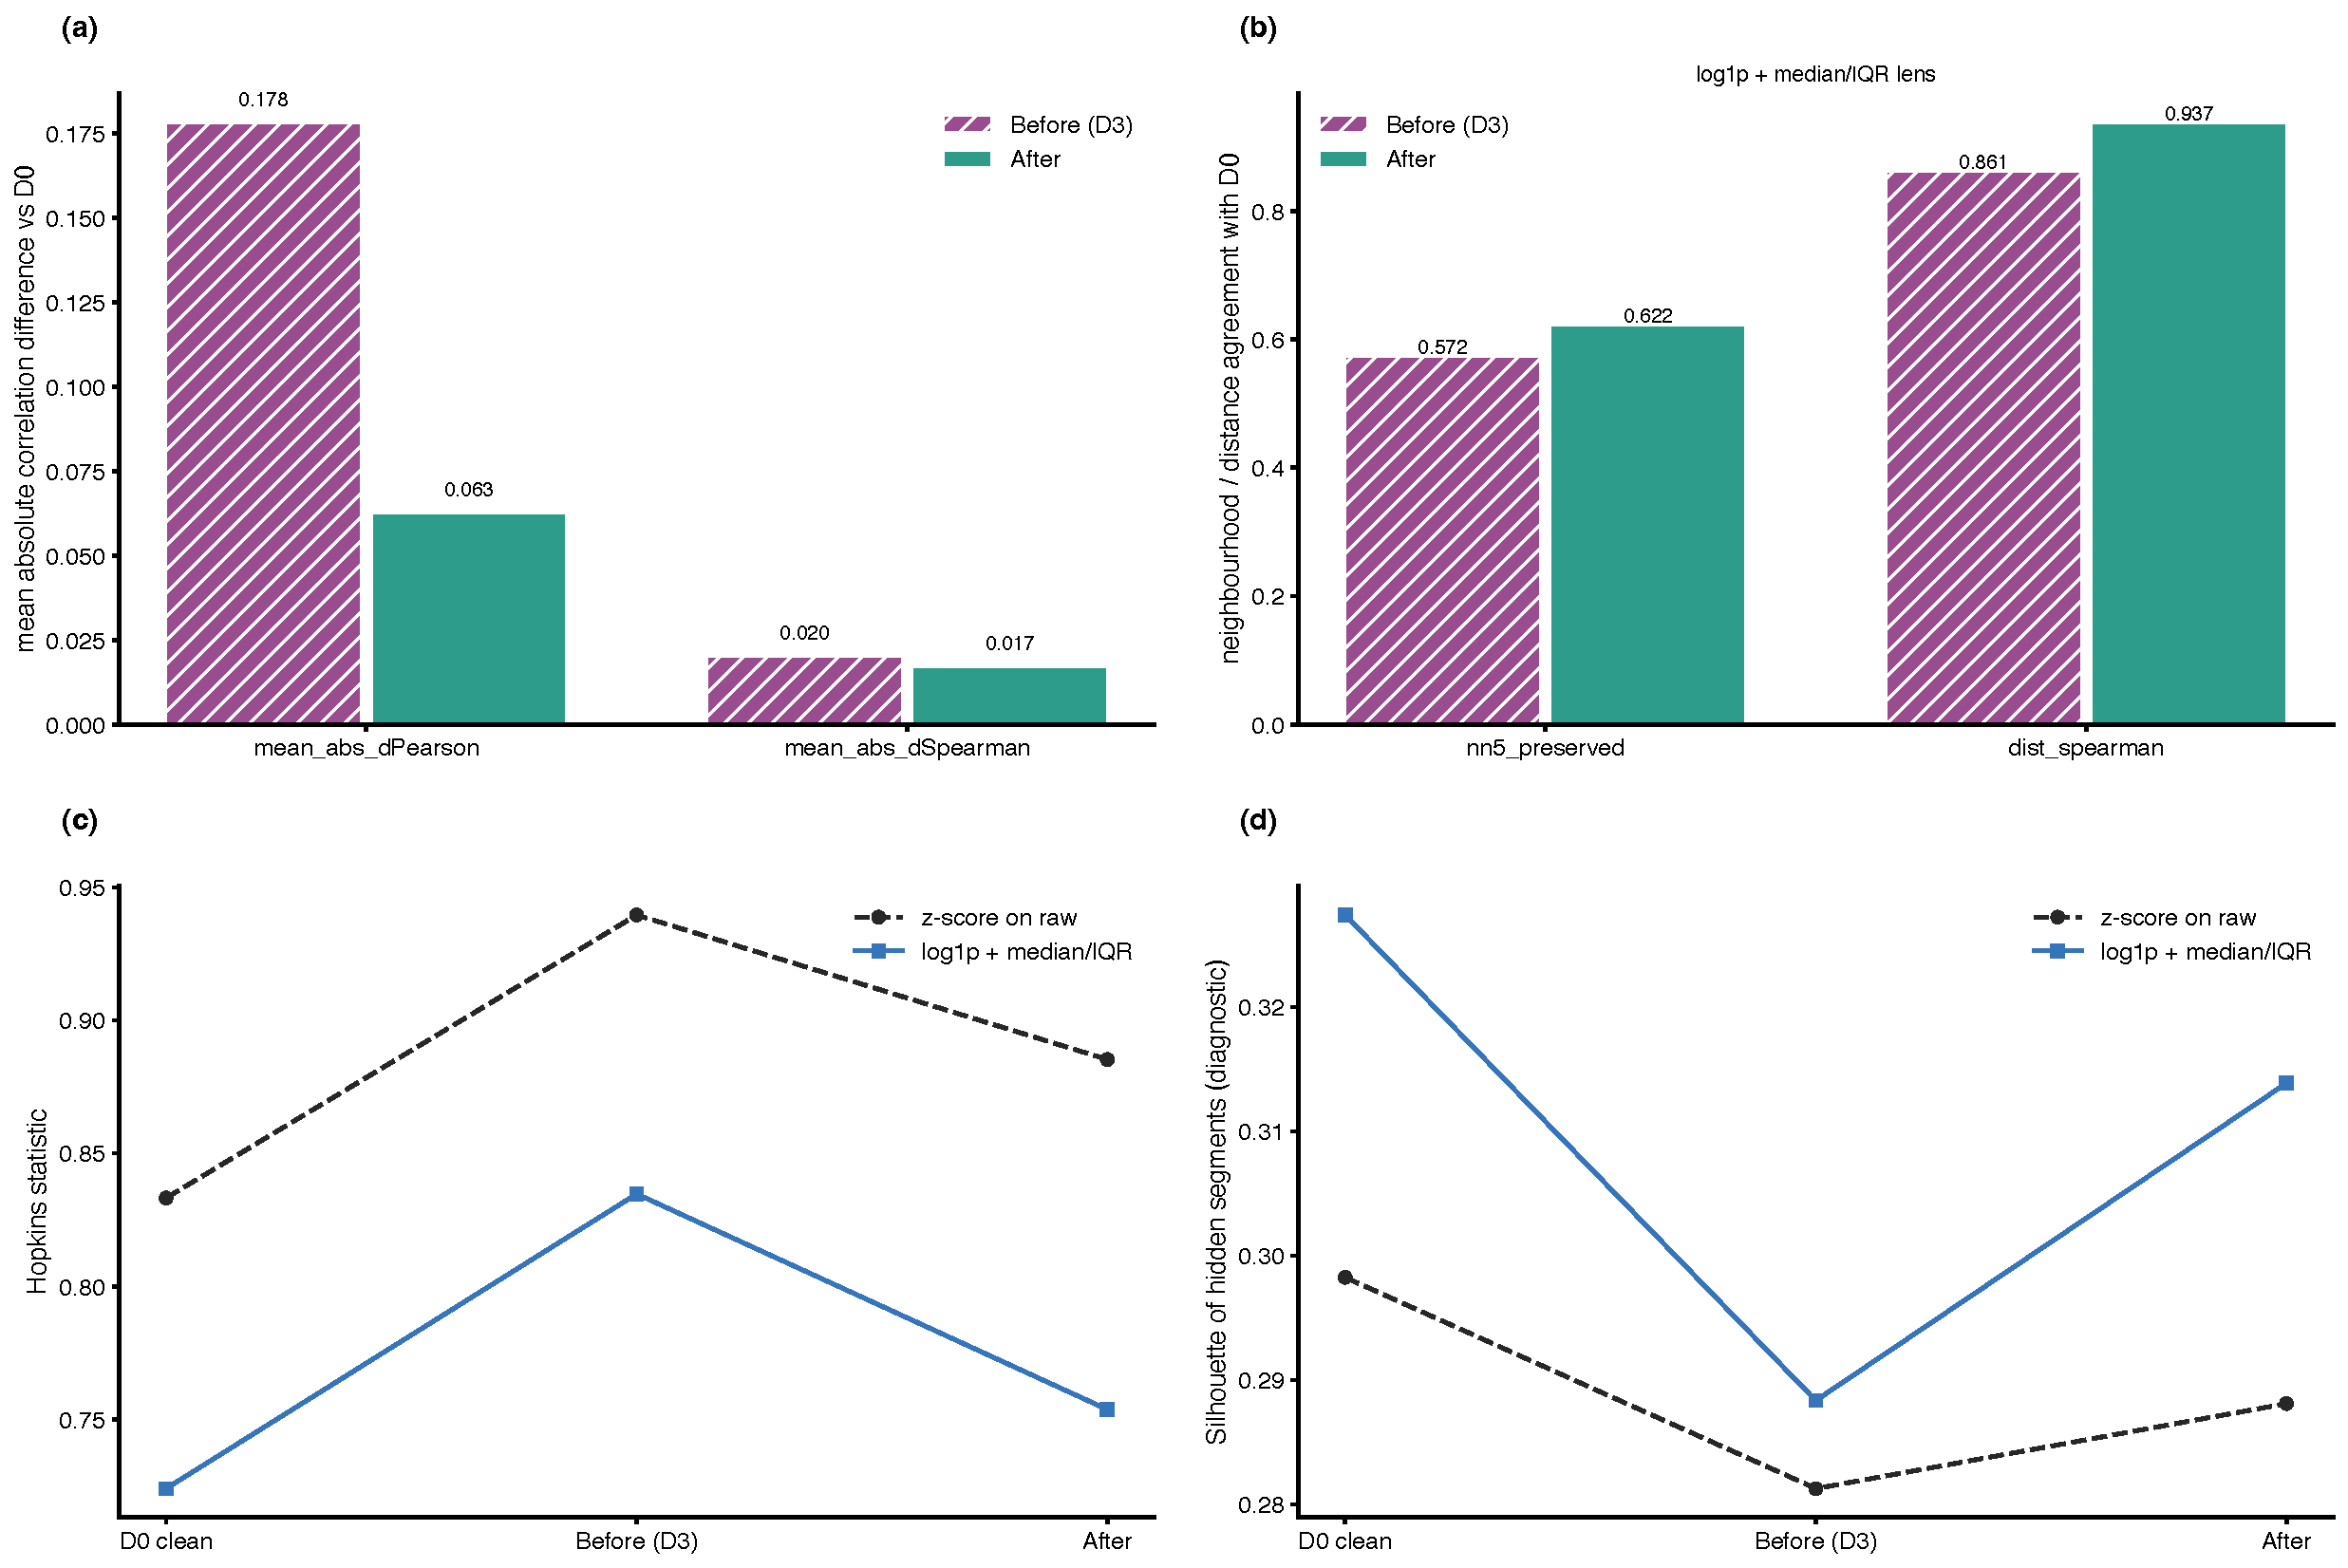
\includegraphics[width=0.92\linewidth]{figE3_structure_vs_clean.pdf}
\caption{Đối chiếu với D0 sau đóng băng (Trước = D3, Sau = đã xử lý). (a) Sai khác tương quan trung bình. (b) Mức giữ lân cận và khoảng cách (log1p + median/IQR).
(c) Hopkins; (d) Silhouette theo nhãn ẩn (chẩn đoán).}
\label{fig:c_eval}
\end{figure}
\FloatBarrier

\section{Câu d: Data Preparation}
\label{sec:d}

Đầu vào là dữ liệu đã xử lý và đóng băng ở câu c (script kiểm tra mã băm trước khi chạy). Mục tiêu là một ma trận số cho thuật toán dựa trên khoảng cách, trong đó mỗi thuộc tính đóng góp một cách có chủ đích.

\subsection{Chuẩn hóa: so sánh StandardScaler, MinMaxScaler và RobustScaler}
Ba bộ chuẩn hóa khác nhau ở thứ được dùng để đặt thang: trung bình và độ lệch chuẩn (Standard), min và max (MinMax), trung vị và IQR (Robust). Với phân cụm dựa trên khoảng cách, điều quan trọng là mỗi cột đóng góp ngang nhau và vài dòng không chi phối.
Trên 10 cột số của dữ liệu đã xử lý (Bảng~\ref{tab:scaler}):
\begin{itemize}
\item \textbf{Standard} làm mỗi cột có phương sai 1 (đúng giả định cân bằng của K-Means) nhưng nhạy với cực trị khi dữ liệu chưa log (17 ô vượt $4$ độ lệch chuẩn).
\item \textbf{MinMax} đặt thang theo min/max nên một cực trị quyết định thang cả cột; vì ta giữ các cực trị hợp lệ, phần lớn khách bị nén vào một đoạn hẹp (cột lớn nhất chiếm 24,7--30,7\% phương sai).
\item \textbf{Robust} bền khi \emph{tính thang} nhưng \emph{không chặn} cực trị: trên dữ liệu thô một khách ``cá voi'' nằm cách 85 đơn vị IQR và 5 dòng chiếm 80,7\% tổng bình phương, nên Robust chỉ phù hợp sau khi đã log.
\end{itemize}
Chọn \textbf{log1p + StandardScaler}: cân bằng nhất (cột lớn nhất 11,9\%, gần $1/10$) và ít bị vài dòng chi phối nhất trong nhóm cột có phương sai bằng nhau. Robust sau log là phương án gần tương đương (không lưu riêng).

\begin{table}[htbp]
\centering\small
\caption{So sánh bộ chuẩn hóa trên 10 cột số (thô hoặc sau log1p). ``5 dòng'' là phần tổng bình phương độ lệch do 5 dòng lớn nhất nắm giữ; ``cột lớn nhất'' là phần phương sai của cột lớn nhất.}
\label{tab:scaler}
\begin{tabular}{lcccc}
\toprule
Biểu diễn & 5 dòng & Cột lớn nhất & $\max|\text{giá trị}|$ & Ô vượt $4$ sd\\
\midrule
thô + Standard & 21,9\% & 11,3\% & 12,7 & 17\\
thô + MinMax & 7,7\% & 30,7\% & 1,0 & 17\\
thô + Robust & 80,7\% & 52,3\% & 85,2 & 17\\
log1p + \textbf{Standard} & \textbf{6,6\%} & \textbf{11,9\%} & 5,8 & 2\\
log1p + MinMax & 4,6\% & 24,7\% & 1,0 & 2\\
log1p + Robust & 8,8\% & 16,9\% & 5,5 & 2\\
\bottomrule
\end{tabular}
\end{table}

\subsection{Mã hóa biến phân loại và vấn đề one-hot chi phối khoảng cách}
Biến thứ tự \var{membership_tier} được mã $0/1/2$ rồi z-score (giữ thứ tự bronze $<$ silver $<$ gold, một cột); biến nhị phân \var{app_installed} chỉ z-score.
Biến định danh \var{device_type} (3 mức) và \var{preferred_category} (5 mức) dùng one-hot. Nếu z-score luôn các cột dummy thì mức hiếm bị khuếch đại: dummy \texttt{unknown} (5\% dòng) có $z=4{,}36$ và khối \var{preferred_category} chiếm 30\% tổng phương sai
dù chỉ là một biến trên 13. Nếu để dummy 0/1 thô thì mỗi biến định danh đóng góp ít hơn một cột số. Giải pháp: giữ dummy 0/1 và nhân với trọng số $w$ sao cho \emph{kỳ vọng bình phương khoảng cách giữa hai khách ngẫu nhiên} của biến đó bằng với một cột số chuẩn hóa.

Với biến định danh có xác suất các mức $p_j$, hai khách khác mức có khoảng cách bình phương $2w^2$ và cùng mức có khoảng cách $0$, nên
\begin{equation}
\mathbb E[d^2] = 2w^2\Big(1-\sum_j p_j^2\Big) \overset{!}{=} 2 \quad\Longrightarrow\quad w = \frac{1}{\sqrt{1-\sum_j p_j^2}} .
\end{equation}
Vế phải $2$ là kỳ vọng $\mathbb E[(z_i-z_j)^2]=2\,\mathrm{Var}(z)$ của một cột z-score. Kết quả: $w_{\mathrm{device}}=1{,}301$, $w_{\mathrm{category}}=1{,}125$ (tính trên 247 nhãn đã biết). Mức \texttt{unknown} được mã bằng hàng toàn số $0$ ở khối category,
tức cách đều mọi nhãn và không tạo trục riêng cho 13 dòng.

\begin{table}[htbp]
\centering\small
\caption{Tỉ trọng phương sai theo khối trong ma trận thiết kế với ba cách mã hóa. Mỗi biến số/hạng/nhị phân/device của mã hóa C đóng góp đúng 7,71\% khoảng cách (category 7,43\%).}
\label{tab:blocks}
\begin{tabular}{lcccc}
\toprule
Mã hóa & Số (9 cột) & Hạng + nhị phân & \var{device_type} & \var{preferred_category}\\
\midrule
A. z-score cả dummy & 45,0\% & 10,0\% & 15,0\% & \textbf{30,0\%}\\
B. dummy 0/1 thô & 72,9\% & 16,2\% & 4,8\% & 6,2\%\\
C. dummy $\times\,w$ (chính) & 69,4\% & 15,4\% & 7,7\% & 7,4\%\\
\bottomrule
\end{tabular}
\end{table}

\subsection{Chọn thuộc tính, giảm chiều và thuật toán}
\paragraph{Thuộc tính dư thừa.} Trên thang log, $R^2$ của $\ln$(\var{total_spend_12m}) theo $\ln$(\var{n_orders_12m}) và $\ln$(\var{avg_order_value}) là $0{,}987$ (VIF $82{,}5$): \var{total_spend_12m} gần như là hàm của hai cột kia theo định nghĩa.
Bỏ nó làm VIF của \var{n_orders_12m} giảm từ $67{,}1$ xuống $7{,}3$ và của \var{avg_order_value} từ $14{,}8$ xuống $2{,}3$. Các cột khác có $R^2\le 0{,}90$ và ý nghĩa nghiệp vụ riêng (ví dụ \var{pages_per_session} VIF $10{,}2$) nên được giữ.
Phiên bản giữ lại \var{total_spend_12m} được lưu riêng (\var{X_full_features}).

\paragraph{PCA.} Giữ 90\% phương sai cần 9 trong 19 thành phần nhưng chỉ bảo toàn $74\%$ lân cận 5-NN so với không gian đầy đủ (5 thành phần chỉ $55\%$): các hướng phương sai thấp mang thông tin cục bộ.
Với $N=260$ và 19 cột không cần giảm chiều để tính toán, và không giảm chiều chỉ để biểu đồ đẹp hơn; PCA 90\% chỉ là biến thể để so sánh (Hình~\ref{fig:d_red}).

\paragraph{K-Means, K-Prototypes hay Gower.} Dữ liệu hỗn hợp nhưng thiên về số: 9 cột số, 1 hạng, 1 nhị phân, 2 định danh (13 thuộc tính sau chọn lọc), và quan hệ của biến phân loại với biến số yếu
(câu b: Cramér $V\le 0{,}24$; $\varepsilon^2$ của thiết bị $\le 0{,}11$). K-Means trên ma trận trên là phương án chính: với $w$, mỗi biến đóng góp ngang nhau, tức đã làm điều mà tham số $\gamma$ của K-Prototypes phải điều chỉnh,
và $\gamma$ không có giá trị ``đúng'' trong học không giám sát. K-Prototypes không chạy được (môi trường không có thư viện \texttt{kmodes}). Thay vào đó lưu ma trận khoảng cách Gower ($260\times260$, bỏ biến khi \texttt{unknown})
cho phân cụm phân cấp; hình học của nó khác $X_{\text{main}}$ rõ (5-NN trùng $0{,}71$, tương quan hạng khoảng cách $0{,}894$).

\subsection{Kết quả chuẩn bị}
Số thuộc tính: \textbf{14 $\to$ 13 $\to$ 19 cột} (bỏ \var{total_spend_12m}; mã hóa tạo 3 + 5 cột one-hot). Ma trận chính $X_{\text{main}}$ gồm: 6 cột log1p + z-score (\var{n_orders_12m}, \var{avg_order_value}, \var{recency_days}, \var{sessions_per_month}, \var{avg_session_minutes}, \var{pages_per_session}),
3 cột z-score (\var{age}, \var{discount_usage_rate}, \var{cart_abandon_rate}), 1 cột hạng, 1 cột nhị phân, 3 cột dummy device và 5 cột dummy category (nhân $w$); 260 hàng, không NaN/inf, không có \var{customer_id} hay cờ metadata.
Độ lệch (skew) sau biến đổi: \var{n_orders_12m} $3{,}33\to0{,}52$, \var{sessions_per_month} $1{,}16\to-0{,}63$, \var{avg_session_minutes} $2{,}07\to0{,}47$, \var{pages_per_session} $1{,}64\to0{,}52$, \var{recency_days} $1{,}67\to-0{,}55$;
\var{avg_order_value} chỉ giảm từ $10{,}92$ xuống $1{,}67$ và vẫn có $z$ lớn nhất $5{,}8$ vì các cực trị hợp lệ được giữ lại.
Tỉ trọng khoảng cách: trước chuẩn bị (số thô, không scale) \var{total_spend_12m} chiếm 99,78\% và mọi cột còn lại gộp 0,22\%; sau chuẩn bị mỗi biến chiếm $\approx 7{,}7\%$ (Hình~\ref{fig:d_enc}).

\begin{figure}[htbp]
\centering
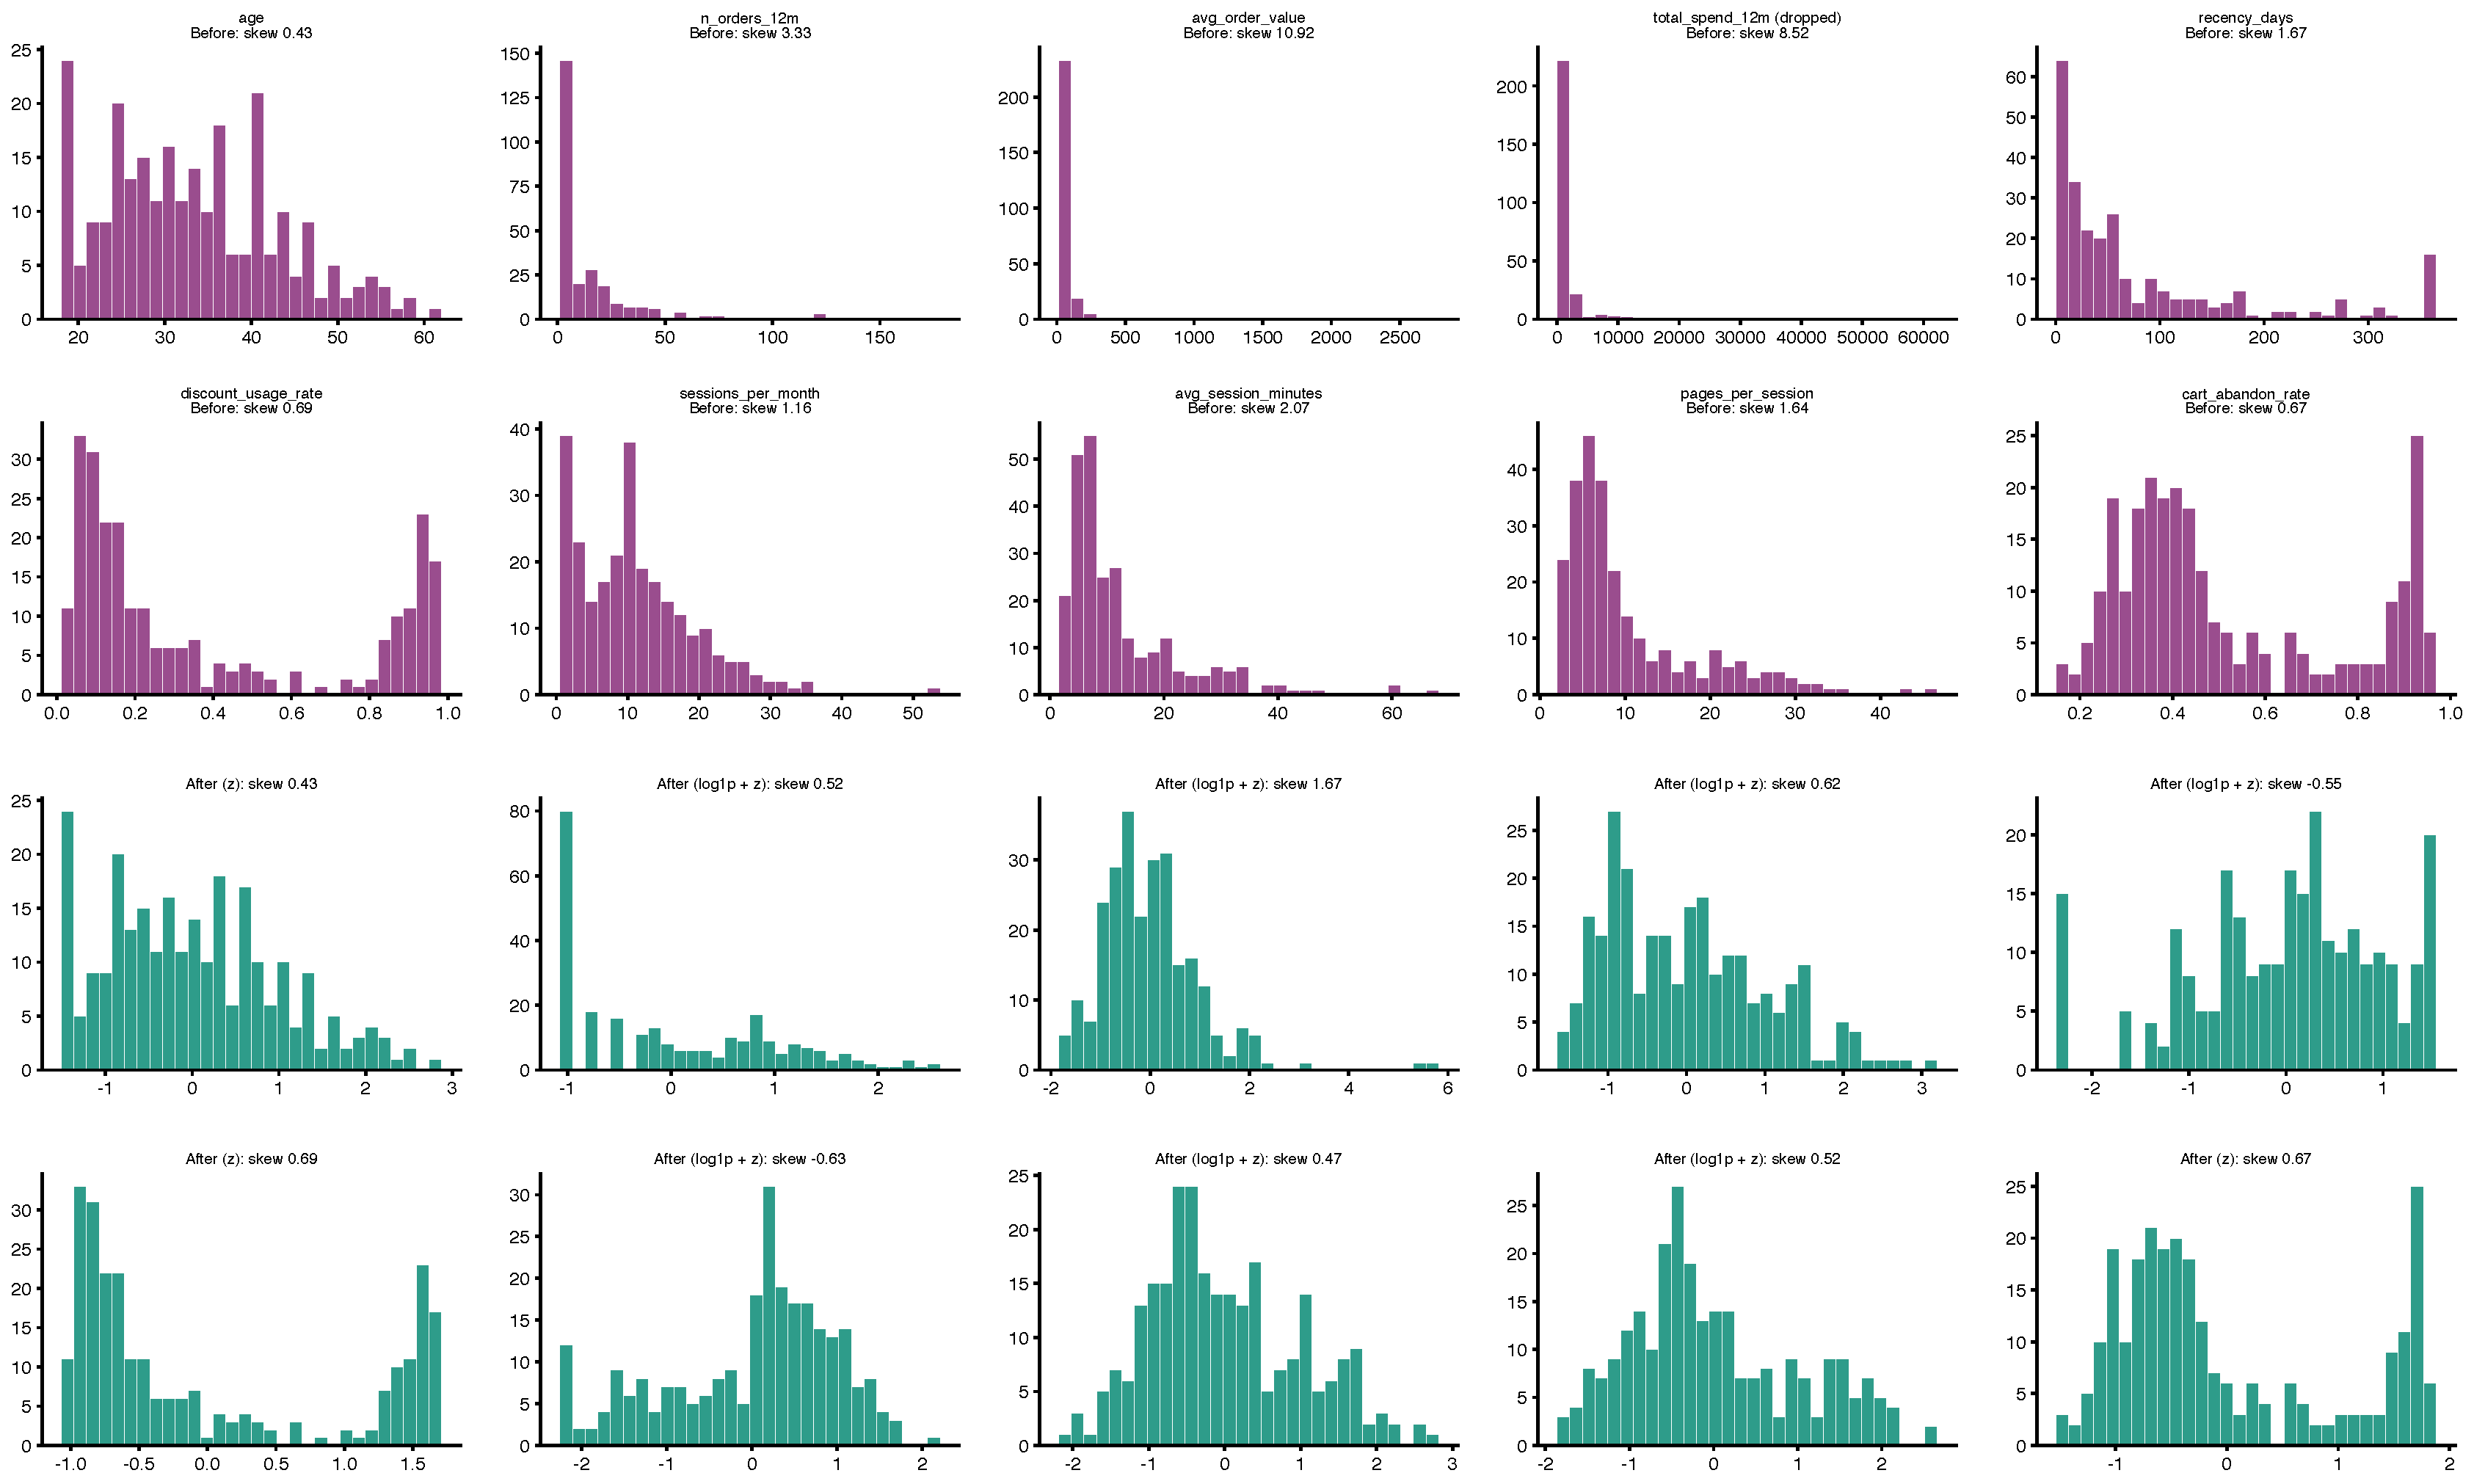
\includegraphics[width=\linewidth]{figD1_distributions_before_after.pdf}
\caption{Phân phối 10 cột số trước (hai hàng trên, tím) và sau chuẩn bị (hai hàng dưới, lam-lục). Cột \var{total_spend_12m} bị loại ở ma trận chính nhưng vẫn hiển thị. Khối cột tại $n=1$ của \var{n_orders_12m} vẫn còn sau log.}
\label{fig:d_dist}
\end{figure}

\begin{figure}[htbp]
\centering
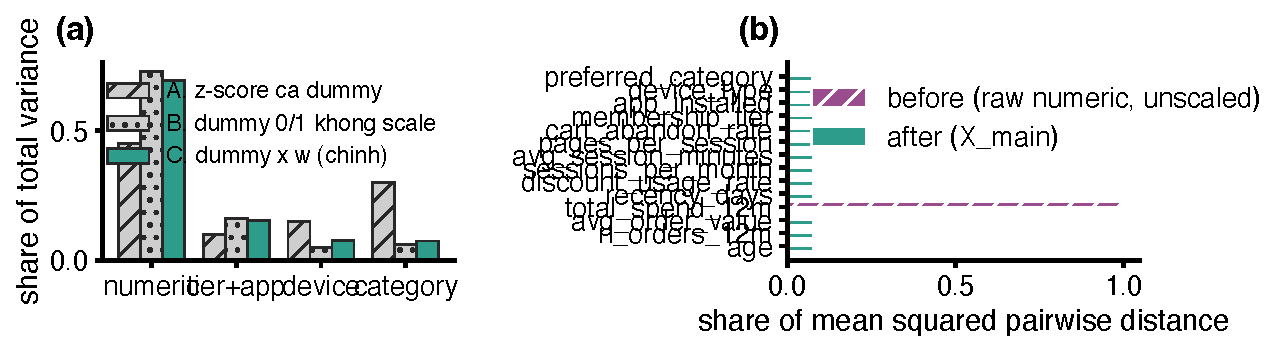
\includegraphics[width=\linewidth]{figD3_encoding_and_distance_share.pdf}
\caption{(a) Tỉ trọng phương sai theo khối với ba cách mã hóa (C là phương án chính). (b) Tỉ trọng bình phương khoảng cách theo thuộc tính gốc: trước chuẩn bị (tím, số thô không scale) và sau (lam-lục).}
\label{fig:d_enc}
\end{figure}

\begin{figure}[htbp]
\centering
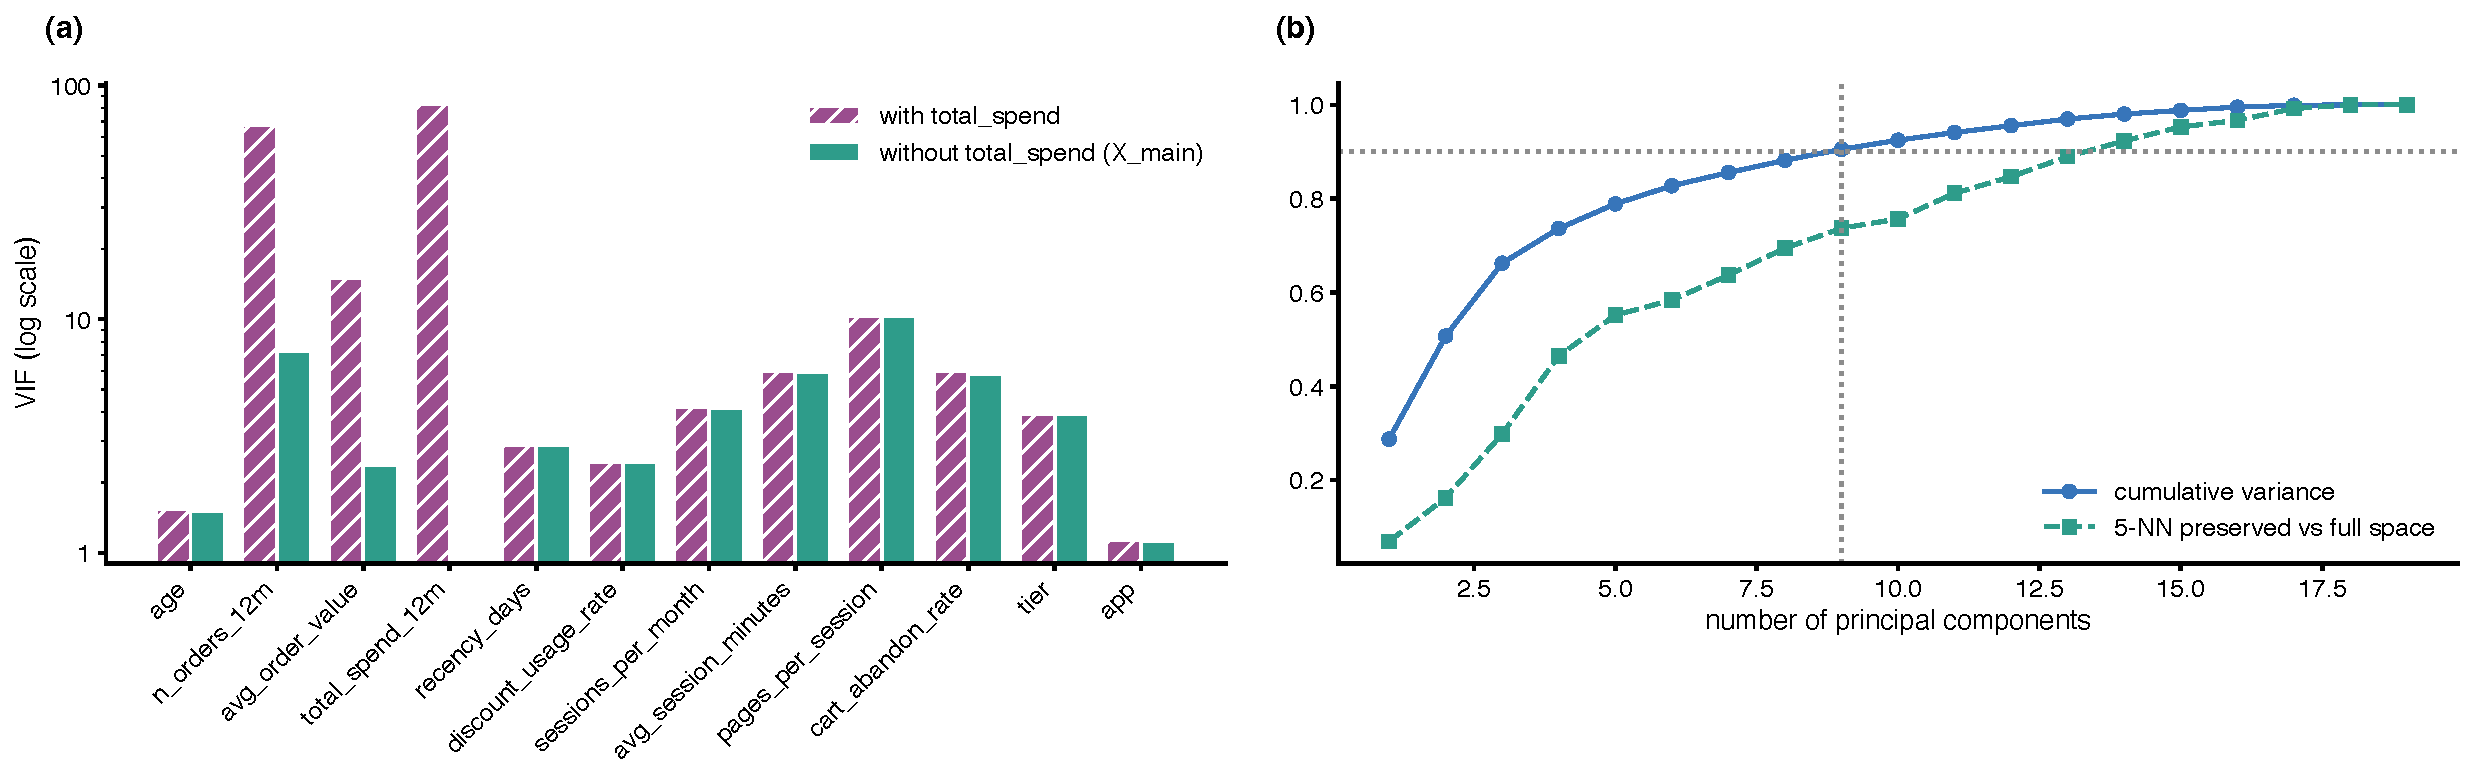
\includegraphics[width=\linewidth]{figD4_redundancy_and_pca.pdf}
\caption{(a) VIF trên thang log khi có và không có \var{total_spend_12m}. (b) Phương sai tích lũy và mức giữ lân cận 5-NN theo số thành phần PCA: 90\% phương sai (9 thành phần) chỉ giữ 74\% lân cận.}
\label{fig:d_red}
\end{figure}

\begin{table}[htbp]
\centering\small
\caption{Các phiên bản ma trận đã lưu và mức đồng thuận hình học với ma trận chính (5-NN trùng; tương quan hạng của khoảng cách cặp).}
\label{tab:variants}
\begin{tabular}{lccc}
\toprule
Phiên bản & Số cột & 5-NN trùng & Tương quan hạng\\
\midrule
\var{full_features} (còn total\_spend) & 20 & 0,939 & 0,993\\
\var{cat_unknown_col} & 20 & 0,966 & $>0{,}999$\\
\var{cat_knn7} & 19 & 0,959 & $>0{,}999$\\
\var{cat_mode} & 19 & 0,941 & $>0{,}999$\\
\var{no_category} & 14 & 0,685 & 0,997\\
\texttt{pca90} & 9 & 0,737 & 0,995\\
Gower (ma trận khoảng cách) & -- & 0,708 & 0,894\\
\bottomrule
\end{tabular}
\end{table}

Bộ biến đổi được lưu bằng sklearn (\texttt{ColumnTransformer}, \texttt{joblib}) cùng siêu dữ liệu từng cột, cấu hình và mã băm; nạp lại trong tiến trình mới tái tạo $X_{\text{main}}$ với sai khác lớn nhất $4{,}4\times10^{-16}$,
và tái dựng tay bằng NumPy cho kết quả khớp. Nghiệm thu 13/13 đạt.
\FloatBarrier

\section{Phân cụm và đánh giá kết quả}
\label{sec:e}

\subsection{Thiết lập thực nghiệm}
\paragraph{Thuật toán.} \textbf{K-Means} (\var{n_init}=50, \var{random_state}=42) là thuật toán chính: khoảng cách Euclid trên ma trận đã chuẩn hóa đúng là điều bước chuẩn bị đã thực hiện, tái lập được và tâm cụm đọc được.
Thuật toán thứ hai là \textbf{phân cụm phân cấp trên khoảng cách Gower} (không cần ma trận số, dùng thang riêng) để xem kết luận có chỉ đúng với K-Means hay không. Chưa dùng DBSCAN/GMM; K-Prototypes không chạy được (thiếu thư viện \texttt{kmodes}).

\paragraph{Các nhánh so sánh.} Cả năm nhánh dùng \textbf{cùng 260 khách}; số cột khác nhau và là một phần của khác biệt cần đọc (Bảng~\ref{tab:branches}). B1 là nền công bằng: biến đổi \emph{tối thiểu} để K-Means chạy
(điền trung vị, one-hot, mã hạng, z-score mọi cột); B0 bỏ cả z-score để thấy riêng tác động của thang đo; L2 là dữ liệu sau tiền xử lý với đúng biến đổi của B1 (tách đóng góp của tiền xử lý khỏi chuẩn bị); L3 là $X_{\text{main}}$ của bước chuẩn bị.
REF là dữ liệu sạch D0 qua đúng pipeline của bước chuẩn bị: \textbf{mốc trần}, không phải một phương pháp.

\begin{table}[htbp]
\centering\small
\caption{Các nhánh so sánh (cùng 260 dòng).}
\label{tab:branches}
\begin{tabularx}{\linewidth}{llcX}
\toprule
Nhánh & Vai trò & Số cột & Dữ liệu và biến đổi\\
\midrule
B0 & Phụ & 20 & D3, điền trung vị, one-hot, mã hạng, \emph{không} chuẩn hóa\\
\textbf{B1} & \textbf{Trước xử lý} & 20 & B0 + z-score mọi cột\\
L2 & Phụ (riêng tiền xử lý) & 21 & Dữ liệu sau tiền xử lý, cùng biến đổi như B1 (\texttt{unknown} là một mức)\\
\textbf{L3} & \textbf{Sau xử lý, chuẩn bị} & 19 & $X_{\text{main}}$ (log1p, z-score, one-hot $\times\,w$, bỏ total\_spend)\\
REF & Mốc trần & 19 & D0 sạch qua đúng pipeline của bước chuẩn bị\\
\bottomrule
\end{tabularx}
\end{table}

\paragraph{Chọn $k$ và chỉ số.} $k$ được chọn \emph{chỉ bằng chỉ số nội tại} (Silhouette cao nhất, $k=2,\dots,8$); nhãn phân khúc ẩn không tham gia chọn $k$, tham số hay biến. Vì 4 là số phân khúc do ta thiết kế, kết quả được báo cáo ở cả $k$ chọn theo nội tại và $k=4$ cố định (để so cùng $k$).
Chỉ số ngoài: ARI, NMI, purity so với phân khúc ẩn. Chỉ số nội tại: Silhouette, Davies--Bouldin, Calinski--Harabasz ở thang riêng \emph{và ở thang chung} $X_{\text{main}}$; chỉ thang chung mới so sánh được giữa các nhánh.
Độ ổn định: ARI giữa cụm trên mẫu con 80\% (30 lần) và cụm đầy đủ; ARI giữa 20 lần chạy \var{n_init}=1 và lần tốt nhất. Khoảng tin cậy 95\% bằng bootstrap 1000 lần theo dòng, ghép cặp giữa các nhánh.

\subsection{Kết quả}
\paragraph{Chọn số cụm.} Trên dữ liệu thô, Silhouette ở thang riêng tăng gần liên tục theo $k$ và B1 chọn $k=7$ (Silhouette $0{,}180$, có một cụm chỉ 1 dòng); L2 cũng chọn $k=7$; B0 chọn $k=2$ với Silhouette $0{,}948$ và cụm $257/3$, một phân hoạch suy biến.
Chỉ L3 có đỉnh rõ tại đúng $k=4$ (Silhouette $0{,}299$; Davies--Bouldin thấp nhất $1{,}277$), như dữ liệu sạch (Hình~\ref{fig:e_k}).

\begin{figure}[htbp]
\centering
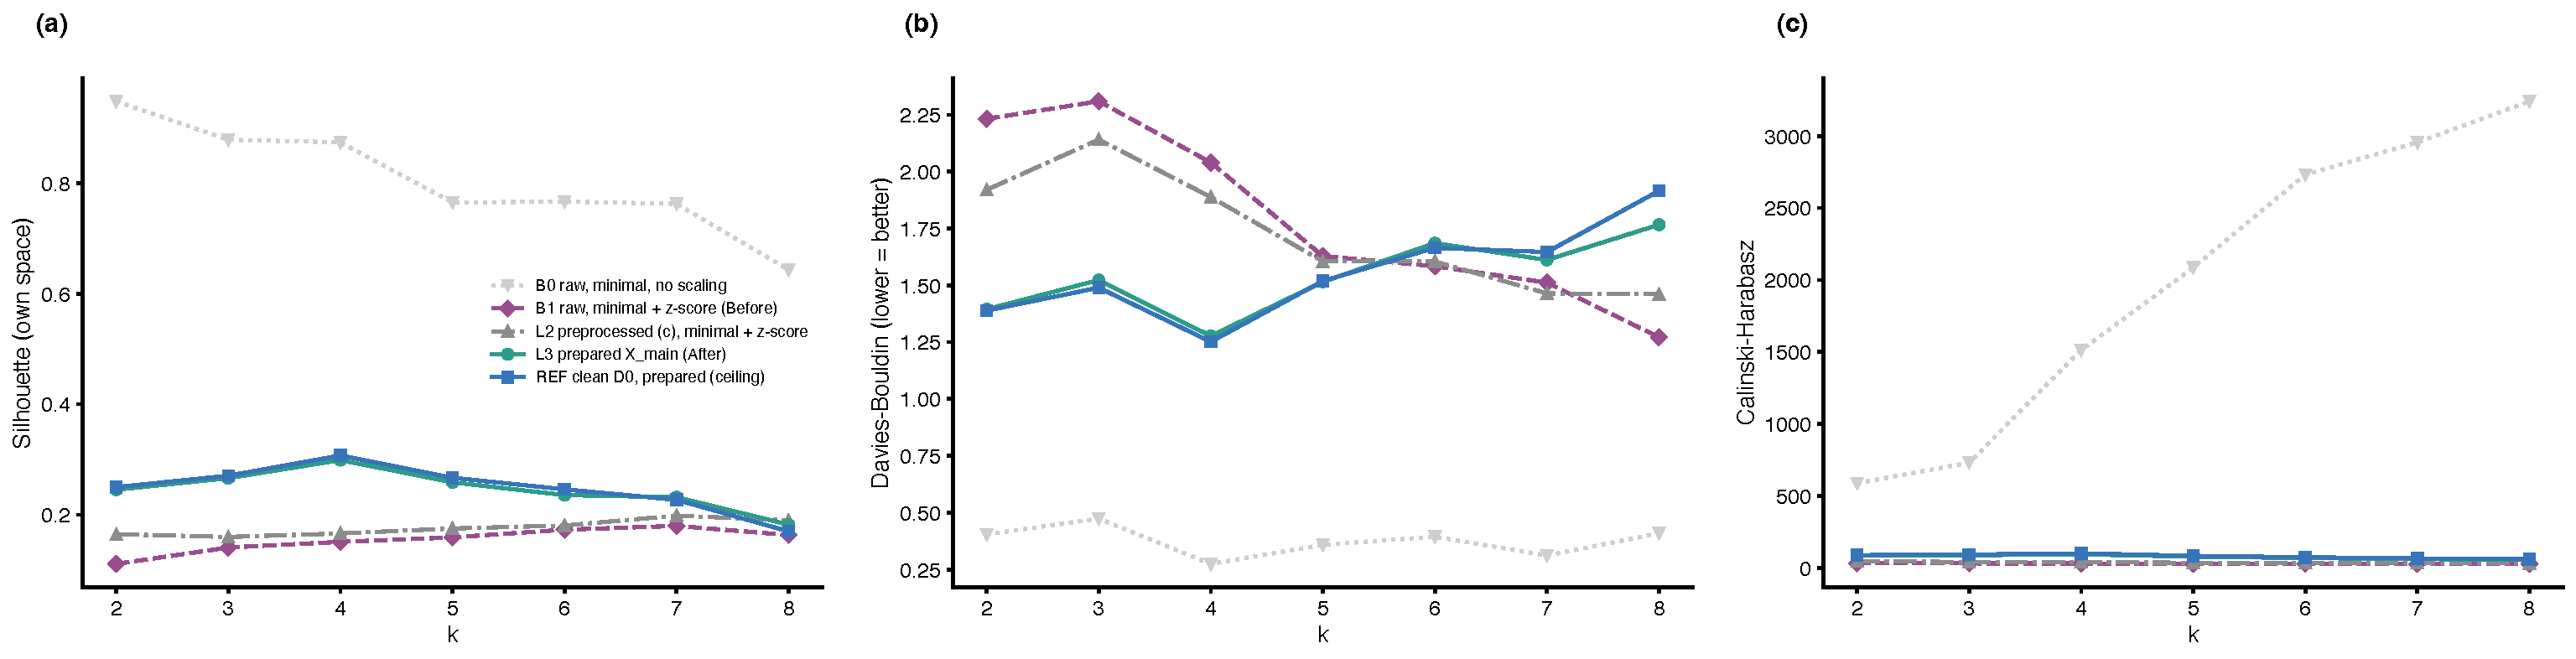
\includegraphics[width=\linewidth]{figE1_k_selection.pdf}
\caption{Chọn $k$ theo Silhouette (cao tốt), Davies--Bouldin (thấp tốt) và Calinski--Harabasz (cao tốt), ở thang riêng của từng nhánh. Giá trị Silhouette thang riêng của B0 (0,95) là của một phân hoạch suy biến.}
\label{fig:e_k}
\end{figure}

\paragraph{Chất lượng phân cụm.} Bảng~\ref{tab:e_k4} và Hình~\ref{fig:e_ext} cho kết quả ở $k=4$. B1 đạt ARI $0{,}611$; sau tiền xử lý (L2) $0{,}701$; sau chuẩn bị (L3) $0{,}745$; dữ liệu sạch (REF) $0{,}777$.
Silhouette ở thang riêng không so sánh được giữa các nhánh (B0 có $0{,}874$ nhưng ARI $0{,}035$); ở thang chung $X_{\text{main}}$ Silhouette tăng từ $0{,}254$ (B1) lên $0{,}299$ (L3) và Davies--Bouldin giảm từ $1{,}449$ xuống $1{,}277$.

\begin{table}[htbp]
\centering\small
\caption{K-Means, $k=4$. ARI có khoảng tin cậy 95\% bootstrap. Ổn định: ARI mẫu con 80\% (trung bình $\pm$ sd) và ARI giữa các lần chạy \var{n_init}=1 (trung bình / thấp nhất).}
\label{tab:e_k4}
\begin{tabular}{lcccccc}
\toprule
Nhánh & ARI [CI 95\%] & NMI & Purity & Sil. thang chung & Kích thước cụm & Ổn định\\
\midrule
B0 & 0,035 \CI{0,016}{0,061} & 0,130 & 0,358 & 0,130 & 245/12/2/1 & 0,914$\pm$0,184; 1,00/1,00\\
\textbf{B1} & \textbf{0,611} \CI{0,515}{0,708} & 0,571 & 0,835 & 0,254 & 82/68/65/45 & 0,829$\pm$0,150; 0,685/0,435\\
L2 & 0,701 \CI{0,610}{0,787} & 0,664 & 0,877 & 0,274 & 82/68/67/43 & 0,949$\pm$0,039; 0,823/0,485\\
\textbf{L3} & \textbf{0,745} \CI{0,658}{0,833} & 0,698 & 0,896 & 0,299 & 77/74/63/46 & 0,970$\pm$0,017; 0,958/0,721\\
REF & 0,777 \CI{0,693}{0,856} & 0,737 & 0,912 & 0,295 & 75/74/66/45 & 0,987$\pm$0,013; 0,996/0,980\\
\bottomrule
\end{tabular}
\end{table}

\begin{figure}[htbp]
\centering
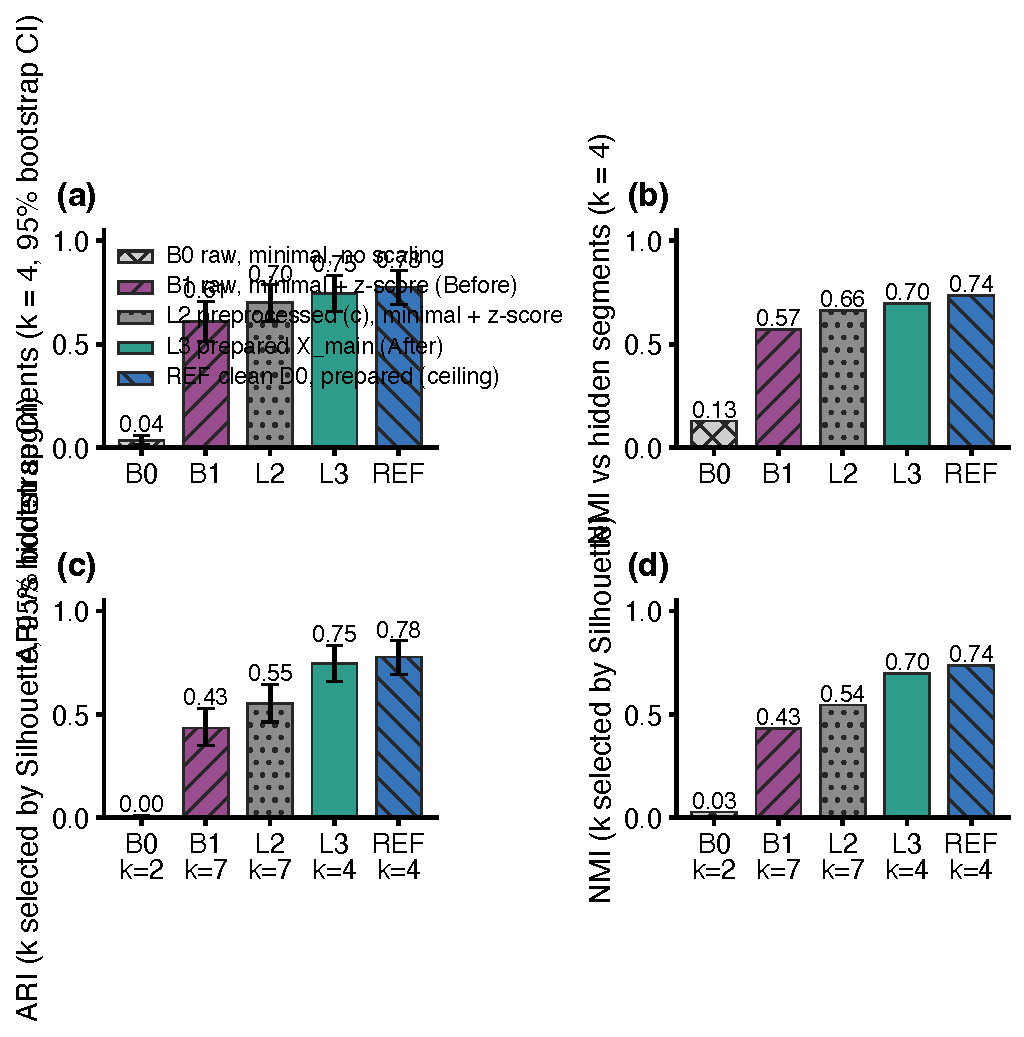
\includegraphics[width=0.9\linewidth]{figE2_external_metrics.pdf}
\caption{Chỉ số ngoài so với phân khúc ẩn. (a, b) ARI (có CI 95\%) và NMI ở $k=4$; (c, d) ARI và NMI khi $k$ chọn theo Silhouette (nhãn trục ghi $k$ được chọn).}
\label{fig:e_ext}
\end{figure}

\paragraph{Chênh lệch có ý nghĩa không?} Bảng~\ref{tab:e_diff} dùng bootstrap ghép cặp. Tổng hiệu quả tiền xử lý + chuẩn bị là rõ ràng ở cả hai thiết lập; riêng tiền xử lý có ý nghĩa; riêng chuẩn bị \emph{không} phân biệt được với 0 ở $k=4$,
và khoảng cách tới dữ liệu sạch cũng không phân biệt được với 0 ở $n=260$.

\begin{table}[htbp]
\centering\small
\caption{Chênh lệch ARI (bootstrap ghép cặp, CI 95\%).}
\label{tab:e_diff}
\begin{tabular}{lcc}
\toprule
So sánh & $k=4$ & $k$ chọn theo Silhouette\\
\midrule
L3 $-$ B1 (tiền xử lý + chuẩn bị) & $+0{,}134$ \CI{0,058}{0,206} & $+0{,}311$ \CI{0,224}{0,393}\\
L2 $-$ B1 (riêng tiền xử lý) & $+0{,}090$ \CI{0,040}{0,143} & $+0{,}117$ \CI{0,057}{0,177}\\
L3 $-$ L2 (riêng chuẩn bị) & $+0{,}044$ \CI{-0,024}{0,115} & $+0{,}194$ \CI{0,101}{0,281}\\
REF $-$ L3 (khoảng cách tới trần) & $+0{,}032$ \CI{-0,007}{0,071} & $+0{,}032$ \CI{-0,007}{0,071}\\
\bottomrule
\end{tabular}
\end{table}

Lợi ích của bước chuẩn bị nằm ở \emph{độ vững} chứ không phải ARI tại $k=4$: L3 chọn đúng $k=4$ trong khi L2 chọn $k=7$ (chênh ARI $+0{,}194$ khi $k$ chọn theo nội tại), và K-Means ít mắc tối ưu cục bộ hơn
(ARI giữa các lần chạy \var{n_init}=1: $0{,}823\to0{,}958$; thấp nhất $0{,}485\to0{,}721$).

\paragraph{Khách ``cầu nối'' quyết định trần.} Trên 213 khách thường, ARI là $0{,}812$ (B1), $0{,}869$ (L2), $\mathbf{0{,}966}$ (L3) và $1{,}000$ (REF); trên 47 khách cầu nối mọi nhánh chỉ đạt $0{,}06$--$0{,}19$ (kể cả REF $0{,}19$).
Phần cải thiện nằm ở khách thường; không phương pháp nào phục hồi được nhóm khách vốn do thiết kế nằm giữa hai phân khúc.

\paragraph{Tác động của dòng hỏng.} Ở $k=4$ trên B1, 7 dòng có ô hỏng không lập thành cụm riêng (cụm nhỏ nhất 45 dòng). Khi $k=7$ (do Silhouette chọn), xuất hiện một cụm chỉ gồm 1 dòng và dòng đó là dòng có ô hỏng. Tác hại chính của ô hỏng là gián tiếp:
làm méo thang đo và làm Silhouette chọn sai $k$.

\subsection{Đặc điểm các cụm}
Ở $k=4$, bốn cụm của L3 tương ứng bốn kiểu khách và khớp tốt với phân khúc ẩn (233/260 khách đúng cụm, 89,6\%; B1: 217/260, 83,5\%).

\begin{table}[htbp]
\centering\small
\caption{Hồ sơ cụm của L3 ($k=4$; trung vị theo đơn vị gốc của dữ liệu đã xử lý) và phân khúc ẩn chiếm đa số.}
\label{tab:e_prof}
\begin{tabularx}{\linewidth}{lrX l}
\toprule
Cụm & $n$ & Đặc điểm (trung vị) & Phân khúc ẩn\\
\midrule
1. Giá trị cao & 46 & 31,5 đơn; tổng chi 3\,093 USD; AOV 110; recency 7 ngày; discount 0,08; hạng gold; mobile; 72\% cài app & HighValue 42/46\\
2. Ít mua & 63 & 2 đơn; tổng chi 114 USD; recency 130 ngày; 2 phiên/tháng; desktop; 43\% cài app & Infrequent 54/63\\
3. Chủ yếu duyệt & 74 & 1 đơn; 17,5 phiên/tháng; 20,7 trang/phiên; bỏ giỏ 0,89; mobile; electronics; 84\% cài app & Browser 66/74\\
4. Săn khuyến mãi & 77 & discount 0,92; 17 đơn; AOV 28; tổng chi 450 USD; fashion; mobile & PromoHunter 71/77\\
\bottomrule
\end{tabularx}
\end{table}

Gợi ý nghiệp vụ suy từ hồ sơ: cụm 1 chăm sóc khách VIP; cụm 2 kích hoạt lại khách đã lâu không mua; cụm 3 tăng chuyển đổi (nhắc giỏ hàng, rút ngắn đường mua); cụm 4 khuyến mãi có kiểm soát biên lợi nhuận.
Với B1, bốn cụm tương tự nhưng lẫn nhiều hơn: 10 khách Infrequent rơi vào cụm khuyến mãi và 6 khách HighValue rơi vào cụm ít mua.

\begin{figure}[htbp]
\centering
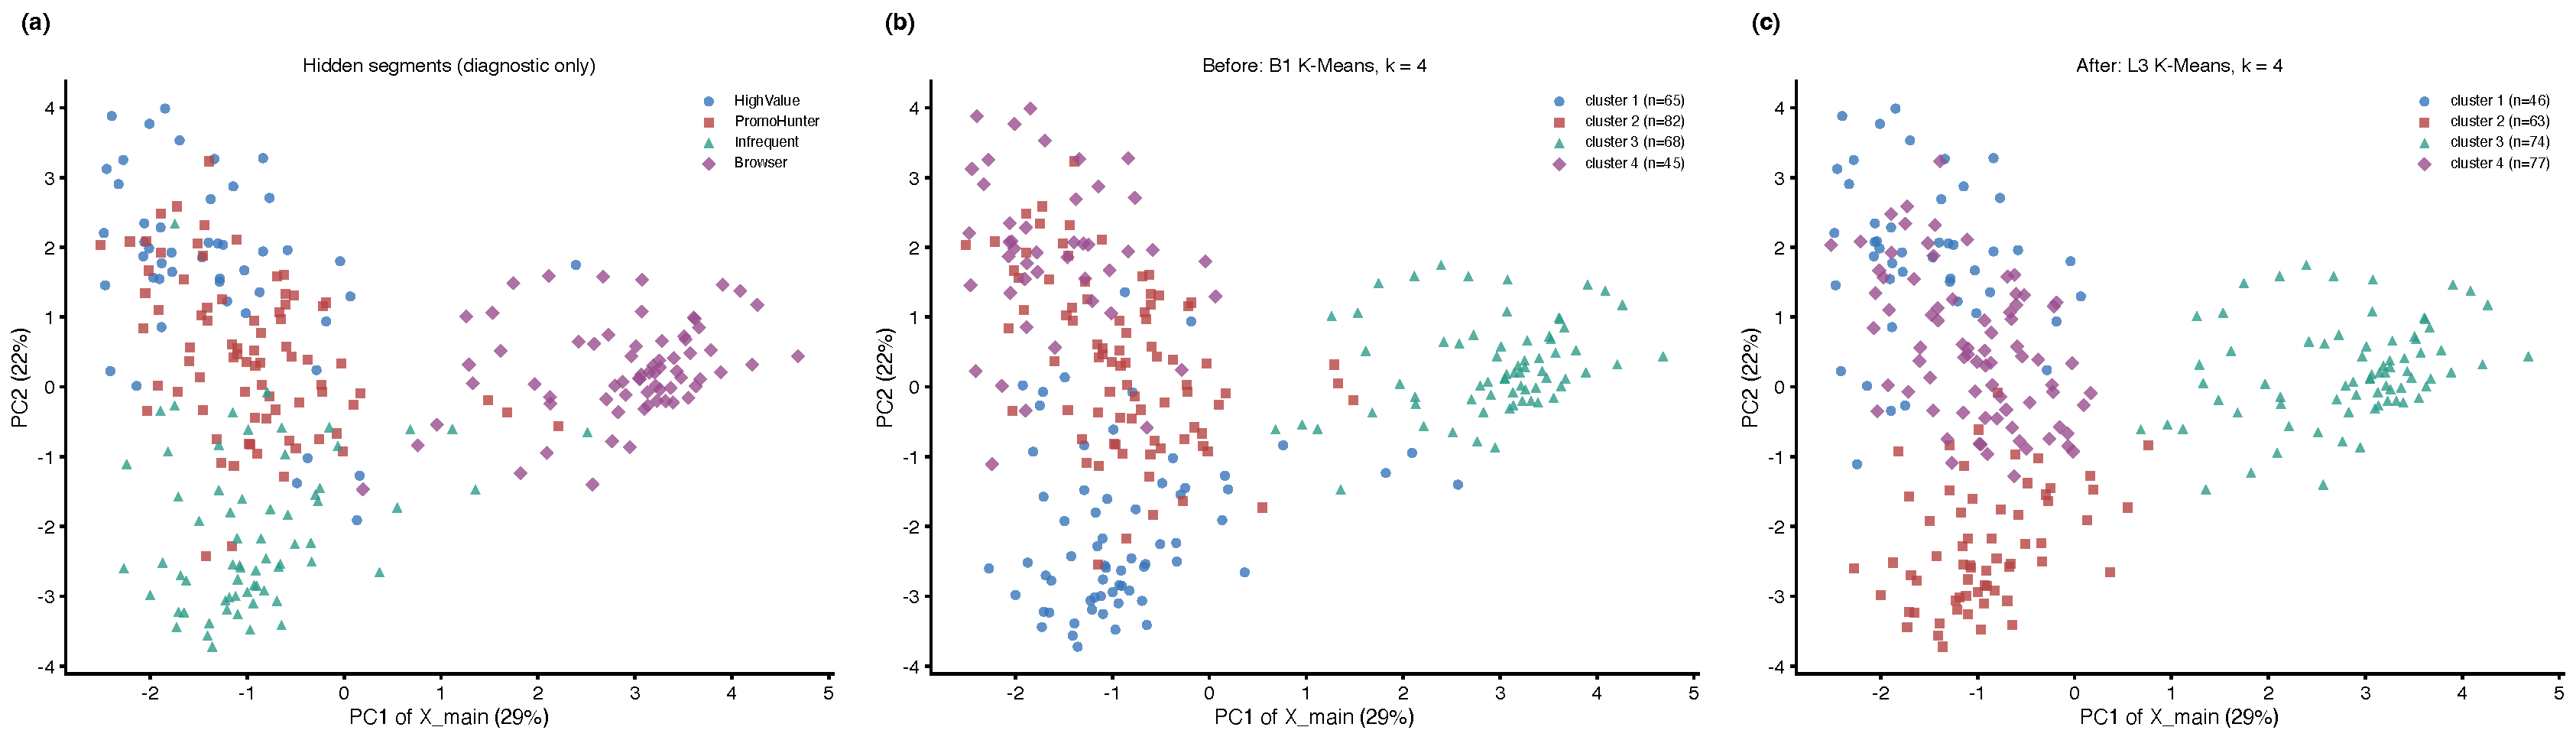
\includegraphics[width=\linewidth]{figE4_pca_embedding.pdf}
\caption{Chiếu PCA 2 chiều của $X_{\text{main}}$: (a) phân khúc ẩn (chỉ chẩn đoán); (b) cụm K-Means của B1 (trước); (c) cụm K-Means của L3 (sau). Cùng một hệ trục nên so sánh trực tiếp được. Màu cụm đặt tùy ý, không tương ứng giữa (b) và (c).}
\label{fig:e_pca}
\end{figure}

\subsection{Thuật toán thứ hai: phân cấp trên khoảng cách Gower}
Liên kết \texttt{average} được chọn trước cho kết quả rất yếu trên dữ liệu thô (cụm $238/18/3/1$). Tôi không chọn lại theo nhãn ẩn; thay vào đó thêm liên kết \texttt{complete} và chọn giữa hai loại \emph{chỉ bằng Silhouette Gower}, in cả hai.
Chỉ số nội tại vẫn chọn nhầm \texttt{average} ở hai nhánh thô. Dù vậy thứ tự B1 $<$ L2 $<$ L3 giống K-Means, nghĩa là kết luận không chỉ đúng với K-Means; mức tuyệt đối thấp hơn nhiều.

\begin{table}[htbp]
\centering\small
\caption{Phân cấp trên khoảng cách Gower ($k=4$); ARI so với phân khúc ẩn. Cột cuối là liên kết được Silhouette Gower chọn.}
\label{tab:gower}
\begin{tabular}{lccc}
\toprule
Nhánh & \texttt{average} (cụm nhỏ nhất) & \texttt{complete} & Được chọn: ARI\\
\midrule
B1 (Gower trên D3 thô) & 0,047 (1 dòng) & 0,126 & average: 0,047\\
L2 (đơn vị gốc, đã xử lý) & 0,170 (1 dòng) & 0,262 & average: 0,170\\
L3 (Gower của bước chuẩn bị) & 0,487 (2 dòng) & 0,605 & complete: 0,605\\
\bottomrule
\end{tabular}
\end{table}

\subsection{Độ nhạy đối với các lựa chọn ở bước tiền xử lý và chuẩn bị}
Bảng~\ref{tab:sens} cho thấy các lựa chọn bị nghi ngờ đều không làm kết quả thay đổi đáng kể ở $k=4$: cách xử lý \texttt{unknown} (thành cột, KNN-7, mode) gần như không ảnh hưởng; bỏ hẳn category đổi khoảng 5\% nhãn và không làm tệ đi;
bỏ \var{total_spend_12m} hay dùng PCA 90\% cũng không đổi đáng kể; loại 34 dòng cực trị hợp lệ không cải thiện, tức giữ chúng không gây hại. Vì vậy quyết định giữ \texttt{unknown} và giữ category không bị bác bỏ, nhưng category cũng không chứng minh được giá trị trên mẫu này.

\begin{table}[htbp]
\centering\small
\caption{Độ nhạy ở $k=4$. Cột ``Chênh'' là chênh ARI so với $X_{\text{main}}$ kèm khoảng tin cậy 95\% (bootstrap ghép cặp); cột cuối là mức đồng thuận ARI với phân cụm chính.}
\label{tab:sens}
\begin{tabular}{lcccc}
\toprule
Biến thể & $N\times$cột & ARI & Chênh [CI 95\%] & Đồng thuận\\
\midrule
$X_{\text{main}}$ & 260$\times$19 & 0,745 & -- & 1,000\\
\var{full_features} (còn total\_spend) & 260$\times$20 & 0,764 & $+0{,}019$ \CI{0,000}{0,048} & 0,979\\
\var{cat_unknown_col} & 260$\times$20 & 0,745 & $0{,}000$ & 1,000\\
\var{cat_knn7} & 260$\times$19 & 0,745 & $0{,}000$ & 1,000\\
\var{cat_mode} & 260$\times$19 & 0,754 & $+0{,}009$ \CI{0,000}{0,027} & 0,989\\
\var{no_category} & 260$\times$14 & 0,771 & $+0{,}026$ \CI{-0,009}{0,066} & 0,948\\
\var{pca90} & 260$\times$9 & 0,746 & $+0{,}001$ \CI{-0,024}{0,029} & 0,979\\
Bỏ 34 dòng cực trị hợp lệ & \textbf{226}$\times$19 & 0,733 & -- & 0,966\\
\bottomrule
\end{tabular}

\smallskip\footnotesize Dòng cuối có số dòng khác (226): để so cùng tập dòng, nhãn của lần chạy đầy đủ trên 226 dòng này cho ARI 0,738.
\end{table}

\section{Kết luận}
\label{sec:concl}

Báo cáo đã xây dựng và kiểm chứng một quy trình phân cụm khách hàng thương mại điện tử từ dữ liệu giả lập đến đánh giá, với các điểm chính sau.
\begin{enumerate}
\item \textbf{Dữ liệu (câu a).} Bộ dữ liệu 260 khách, 14 thuộc tính theo mô hình nhân quả nhiều tầng, 4 phân khúc ẩn có chồng lấn, bốn cột nhiễu, 15 khách có ngoại lai (8 hợp lệ, 7 lỗi) và ba cột thiếu, tái lập được và có nhật ký từng ô bị thay đổi.
\item \textbf{Hiểu dữ liệu (câu b).} Hai vấn đề chi phối hình học khoảng cách là ô hỏng/thang đo và phân phối lệch phải; Pearson bị ô hỏng phá hủy trong khi Spearman bền; thống kê Hopkins bị phồng bởi ngoại lai; phương pháp phát hiện ngoại lai thống kê chung có precision thấp ($0{,}14$) nên không dùng để xóa.
\item \textbf{Tiền xử lý (câu c).} Chỉ sửa từng ô không hợp lệ, điền khuyết theo thí nghiệm che ô có so sánh ghép cặp và quy tắc 1-SE, giữ \texttt{unknown} cho biến định danh có bất định cao, không khử nhiễu từng giá trị, chỉ đánh dấu cực trị hợp lệ. Đối chiếu sau đóng băng cho thấy cải thiện cấu trúc (sai khác Pearson với D0 giảm từ $0{,}178$ xuống $0{,}063$), kèm vài kết quả không thuận lợi được nêu rõ.
\item \textbf{Chuẩn bị (câu d).} Ma trận $260\times19$ với log1p + StandardScaler, one-hot nhân trọng số $w=1/\sqrt{1-\sum p^2}$ để mỗi biến đóng góp ngang nhau, bỏ \var{total_spend_12m} do dư thừa ($R^2=0{,}987$), không PCA ở ma trận chính.
\item \textbf{Phân cụm (câu e).} Ở $k=4$, ARI so với phân khúc ẩn tăng từ $0{,}611$ (trước) lên $0{,}745$ (sau); khi $k$ chọn theo Silhouette, dữ liệu thô cho $k=7$ (ARI $0{,}434$) còn dữ liệu đã chuẩn bị chọn đúng $k=4$ (ARI $0{,}745$) và ổn định hơn rõ rệt (chạy lặp $0{,}685\to0{,}958$).
Phần đóng góp riêng của chuẩn bị tại $k=4$ chưa chứng minh được; bằng chứng nằm ở chọn $k$ và độ vững.
\end{enumerate}

\appendix
\section{Khai báo công cụ AI và nhật ký cộng tác}
\label{app:ai}

\subsection{Công cụ đã dùng}
\begin{itemize}
\item \textbf{Claude Code} (mô hình Claude Sonnet 5.5): đề xuất thiết kế, viết mã, chạy kiểm tra, phân tích kết quả và soạn tài liệu, theo từng giai đoạn: mỗi giai đoạn hoàn thành và kiểm tra thực tế trước khi sang giai đoạn sau.
\item \textbf{Phần mềm}: Python 3.12, NumPy 2.5.1, pandas 2.2.3, scikit-learn 1.9.0, SciPy 1.18.0, Matplotlib 3.11.2; biên dịch báo cáo bằng \texttt{tectonic} (XeTeX), phông TeX Gyre.
\item \textbf{Phong cách biểu đồ}: theo quy ước của repo \emph{figures4papers} (đọc qua công cụ tóm tắt nên không phải bản chép nguyên văn); bảng màu gốc của repo trượt kiểm tra màu (xanh \texttt{\#0F4D92} quá tối, \texttt{\#42949E} quá xám) nên dùng \texttt{\#3775BA} và \texttt{\#2E9C8A} trong cùng họ màu, và thứ tự bốn màu được cố định theo bộ đạt kiểm tra.
\item Lịch sử hội thoại chính với AI được nộp kèm theo (file riêng); nhật ký quyết định đầy đủ gồm 31 mục nằm ở \var{docs/ai_log.md}.
\end{itemize}

\subsection{Cách kiểm chứng sản phẩm của AI}
Mọi kết luận trong báo cáo được rút từ số đo thực chạy; mọi script có kiểm tra nghiệm thu tự động (42, 15, 13 kiểm tra cho câu a, c, d) và chạy lại cho kết quả giống hệt (so mã băm); các hình đều được mở và xem bằng mắt (nhiều lỗi bố cục chỉ lộ khi xem hình);
bước đánh giá với dữ liệu sạch chỉ chạy sau khi kết quả đã đóng băng.

\subsection{Những chỗ AI sai hoặc được chỉnh sửa}
\begingroup\small
\begin{longtable}{>{\raggedright\arraybackslash}p{1.1cm}>{\raggedright\arraybackslash}p{7.3cm}>{\raggedright\arraybackslash}p{6.4cm}}
\caption{Các sửa đổi chính (trích từ \var{docs/ai_log.md}; mục đầy đủ có đánh số).}\label{tab:ailog}\\
\toprule
Câu & Vấn đề & Cách xử lý\\
\midrule
\endfirsthead
\toprule
Câu & Vấn đề & Cách xử lý\\
\midrule
\endhead
\bottomrule
\endfoot
a & Thiết kế đầu quá dễ (ARI sạch 0,98); mô hình nhân quả đầu lại quá khó (ARI 0,47). & Hiệu chỉnh trên dữ liệu sạch; không nới ngưỡng ``một thuộc tính đơn lẻ'' khi thấy $0{,}72>0{,}70$ mà chỉnh dữ liệu.\\
a & Kiểm tra ``nhiễu không thiên lệch'' dùng trung bình của tỉ số (sai phương pháp); ngoại lai ``đại lý'' không cực trị; ``cá voi'' 309 đơn với 36 phiên/tháng (phi nghiệp vụ, bộ kiểm tra không bắt được). & Sửa phép kiểm tra; đặt cường độ theo hàng rào Tukey; thêm kiểm tra số đơn $\le$ 1 đơn/phiên.\\
chung & Sinh viên hai lần dán nhầm đề dạng giám sát (dự đoán \var{purchased_Y}). & AI nêu xung đột, không tạo nhãn mục tiêu, giữ bài toán không giám sát.\\
b & Quy tắc chọn cột cần log chọn nhầm hai biến tỉ lệ; $\chi^2$ cho biến thiếu dùng số kỳ vọng $<5$; trung bình theo thiết bị bị một dòng 1440 phút làm méo. & Đổi quy tắc (ghi nhận là đổi sau khi xem); kiểm định hoán vị (kết luận từ ``có ý nghĩa'' thành ``chưa đủ bằng chứng''); dùng trung vị.\\
b & Thanh màu đè lên panel, chú giải đè lên cột, nhãn log chồng nhau, trục PCA lật dấu. & Chỉ lộ khi xem hình; sửa bố cục.\\
c & Gán $\mathrm{AOV}=\mathrm{total}/n$ cho C0062 (sinh viên đặt điều kiện: chỉ khi từ điển xác nhận đẳng thức chính xác). & Từ điển ghi ``$\sim$'' nên không gán; điền bằng mô hình.\\
c & Kiểm tra ``cực trị không bị sửa'' viết ở mức dòng (trượt oan); ngưỡng ``lặp tối đa 3 lần'' tùy tiện. & Đổi sang mức ô; thay bằng bootstrap p95 (đổi sau khi thấy trượt; dữ liệu không đổi).\\
c & Ước lượng che ô lạc quan cho thời lượng phiên (3,04 so với 3,79 phút thực đo); ô \texttt{recency} của C0242 điền sai (210 so với 69). & Ghi vào hạn chế; không đổi quy trình theo dữ liệu sạch (chống rò rỉ).\\
d & Sinh viên nói đã thống nhất phương án khi chưa xem đề xuất; so khớp tên cột bằng chuỗi con làm sai bảng tỉ trọng khoảng cách của \texttt{age}. & AI nêu rõ đây là lựa chọn của AI để bác bỏ khi review; sửa so khớp và thêm 2 kiểm tra (13/13).\\
e & Liên kết \texttt{average} của phân cấp Gower cho kết quả rất yếu; Silhouette thang riêng của B0 cao (0,95) với ARI 0,005; kỳ vọng ``câu d cải thiện hơn câu c'' không được ủng hộ ở $k=4$. & Thêm \texttt{complete} và chọn bằng chỉ số nội tại, in cả hai; so ở thang chung; ghi đúng kết quả đo.\\
\end{longtable}
\endgroup
\FloatBarrier

\section{Sản phẩm nộp và cách tái lập}
\label{app:repro}

\begin{table}[htbp]
\centering\footnotesize
\caption{Đối chiếu với danh mục sản phẩm của đề.}
\label{tab:deliver}
\begin{tabularx}{\linewidth}{>{\raggedright\arraybackslash}p{4.2cm}X}
\toprule
Sản phẩm & Vị trí trong kho mã\\
\midrule
Báo cáo & \texttt{reports/latex/main.pdf} (nguồn \texttt{main.tex} và các \texttt{sec*.tex})\\
Dữ liệu ban đầu và sau nhiễu, ngoại lai & \var{data/01_generated/}: \var{data_clean_reference.csv} (D0), \var{data_after_noise.csv} (D1), \var{data_after_outliers.csv} (D2), \var{data_raw_corrupted.csv} (D3), \var{data_dictionary.csv}; nhật ký chèn lỗi và nhãn ẩn ở \texttt{data/hidden/}\\
Dữ liệu sau tiền xử lý và chuẩn bị & \var{data/02_preprocessed/} (dữ liệu, nhật ký ô thay đổi, cờ, biến thể, \var{FROZEN_SHA256.json}); \var{data/03_prepared/} (\var{X_main.csv}, \texttt{pipeline/}, \texttt{variants/}); \var{data/04_clustering/} (nhãn cụm, tâm cụm, cấu hình)\\
Mã nguồn và bằng chứng thực nghiệm & \var{src/01_generate_data.py}, \var{02_data_understanding.py}, \var{03_preprocess.py}, \var{03b_evaluate_preprocessing.py}, \var{04_prepare.py}, \var{05_cluster.py}, \var{dm_utils.py}, \var{viz_style.py}; \texttt{notebooks/} (Colab cho câu a); log ở \texttt{logs/}; bảng ở \texttt{reports/tables/}; hình ở \texttt{figures/}\\
Lịch sử hội thoại và khai báo công cụ & Phụ lục~\ref{app:ai}; \var{docs/ai_log.md}; file hội thoại đầy đủ nộp kèm\\
\bottomrule
\end{tabularx}
\end{table}

\paragraph{Chạy lại toàn bộ (CPU, vài phút).} Hạt giống cố định (42); các script ghi log vào \var{logs/}; mọi bước sau câu c từ chối chạy nếu dữ liệu đầu vào không khớp mã băm đã đóng băng.
{\footnotesize
\begin{verbatim}
pip install -r requirements.txt
python src/01_generate_data.py          # câu a (42 kiểm tra nghiệm thu)
python src/02_data_understanding.py     # câu b
python src/03_preprocess.py             # câu c (15 kiểm tra, đóng băng SHA-256)
python src/03b_evaluate_preprocessing.py  # chỉ chạy khi mã băm khớp
python src/04_prepare.py                # câu d (13 kiểm tra)
python src/05_cluster.py                # câu e
cd reports/latex && tectonic main.tex   # biên dịch báo cáo
\end{verbatim}}


\end{document}
